\documentclass[xcolor=pdftex,dvipsnames,table,aspectratio=169]{UT}
\usepackage[utf8]{inputenc}
\usepackage{groove2tikz}
\usepackage{pifont}
\usepackage{amsthm, amsmath, amssymb}
\usepackage{ulem}

\newtheoremstyle{break}{\baselineskip}{0.5\baselineskip}{\itshape}{}{\bfseries}{}{\newline}{}

\theoremstyle{break}
\newtheorem{thm}{Theorem}[section]
\newtheorem{cor}[thm]{Corollary}
\newtheorem{lem}[thm]{Lemma}
%\theoremstyle{definition}
\newtheorem{defin}[thm]{Definition}

\lstset{ %
basicstyle=\footnotesize,       % the size of the fonts that are used for the code
numbers=left,                   % where to put the line-numbers
numberstyle=\footnotesize,      % the size of the fonts that are used for the line-numbers
stepnumber=2,                   % the step between two line-numbers. If it's 1 each line will be numbered
numbersep=5pt,                  % how far the line-numbers are from the code
backgroundcolor=\color{white},  % choose the background color. You must add \usepackage{color}
showspaces=false,               % show spaces adding particular underscores
showstringspaces=false,         % underline spaces within strings
showtabs=false,                 % show tabs within strings adding particular underscores
frame=single,			% adds a frame around the code
tabsize=2,			% sets default tabsize to 2 spaces
captionpos=b,			% sets the caption-position to bottom
breaklines=true,		% sets automatic line breaking
breakatwhitespace=false,	% sets if automatic breaks should only happen at whitespace
escapeinside={\%*}{*)}          % if you want to add a comment within your code
}

\addbibresource{report.bib}

\DeclareGraphicsExtensions{.pdf,.png}
\dominitoc

% Define bijection symbol as defined in the oz package.
% We cannot include the oz package directly because of double definitions. This is a work-around.
\let \tfun \rightarrow
\let \tinj \rightarrowtail
\def \bij {\mathrel{\ooalign{$\tinj$\hfil\cr$\mkern5mu\tfun$}}}

\DeclareMathSymbol{\mstar}{\mathord}{symbols}{"03}
\DeclareMathOperator{\sat}{sat}
\DeclareMathOperator{\new}{\mathbf{new}}
\DeclareMathOperator{\prefix}{\#}
\DeclareMathOperator{\append}{@\:}
\newcommand\type[1]{\mathsf{#1}}

\newcommand\isabelleref[2]{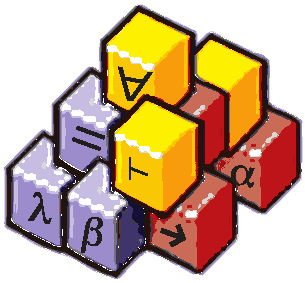
\includegraphics[height=0.75\baselineskip,keepaspectratio]{images/isabelle_logo.pdf} \texttt{\detokenize{#1}} in \texttt{\detokenize{#2}}}
\newcommand\isabellelref[2]{\begin{flushright}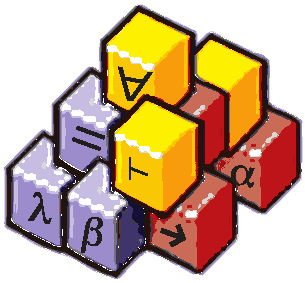
\includegraphics[height=0.75\baselineskip,keepaspectratio]{images/isabelle_logo.pdf} Also see \emph{\texttt{\detokenize{#1}}} in \emph{\texttt{\detokenize{#2}}}\end{flushright}}

\usetikzlibrary{arrows.meta}
\tikzstyle{data}=[rectangle split,rectangle split parts=2,draw,text centered]

\isabellestyle{it}
%\bibliographystyle{acm}

% Custom todo commands
\newcommand\writingtask[1]{\todo[inline]{\textbf{Writing task}: #1}}
\newcommand\missingref[1]{\todo[inline, inlinewidth=2.1cm, noinlinepar, nolist, color=gray!40, size=\tiny]{Missing reference}\todo[color=gray!40, caption={\textbf{Reference missing}: #1}]{#1}}
\newcommand\spellcheck[1]{\todo[color=green!70]{\textbf{Grammar and spellcheck}: #1}}
\newcommand\feedback[1]{\todo[color=blue!70]{\textbf{Proposed feedback}: #1}}

\begin{document} 

\maketitleslide

\setbeamertemplate{background}{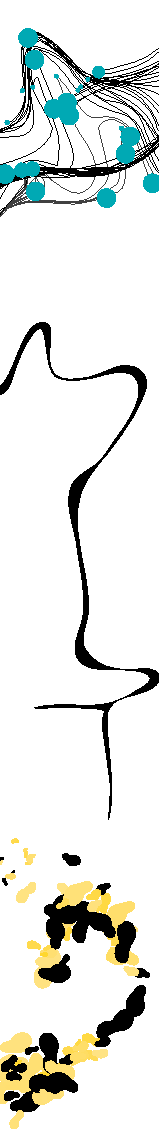
\includegraphics[width=0.08\paperwidth,height=\paperheight]{images/side}}

\section*{Introduction}

\begin{frame}{Introduction}
\begin{columns}[c]
    \begin{column}{0.05\textwidth}
    \end{column}\begin{column}{0.3\textwidth}
        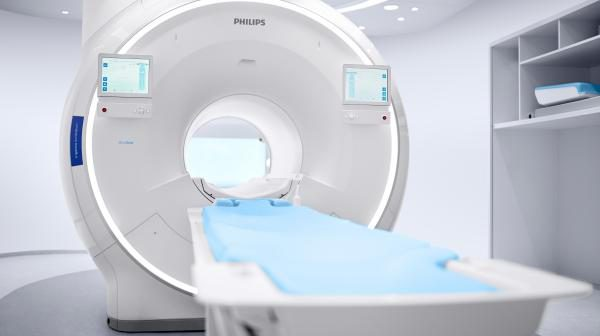
\includegraphics[width=\textwidth]{images/01_introduction/mri.jpg}
    \end{column}\begin{column}{0.3\textwidth}
        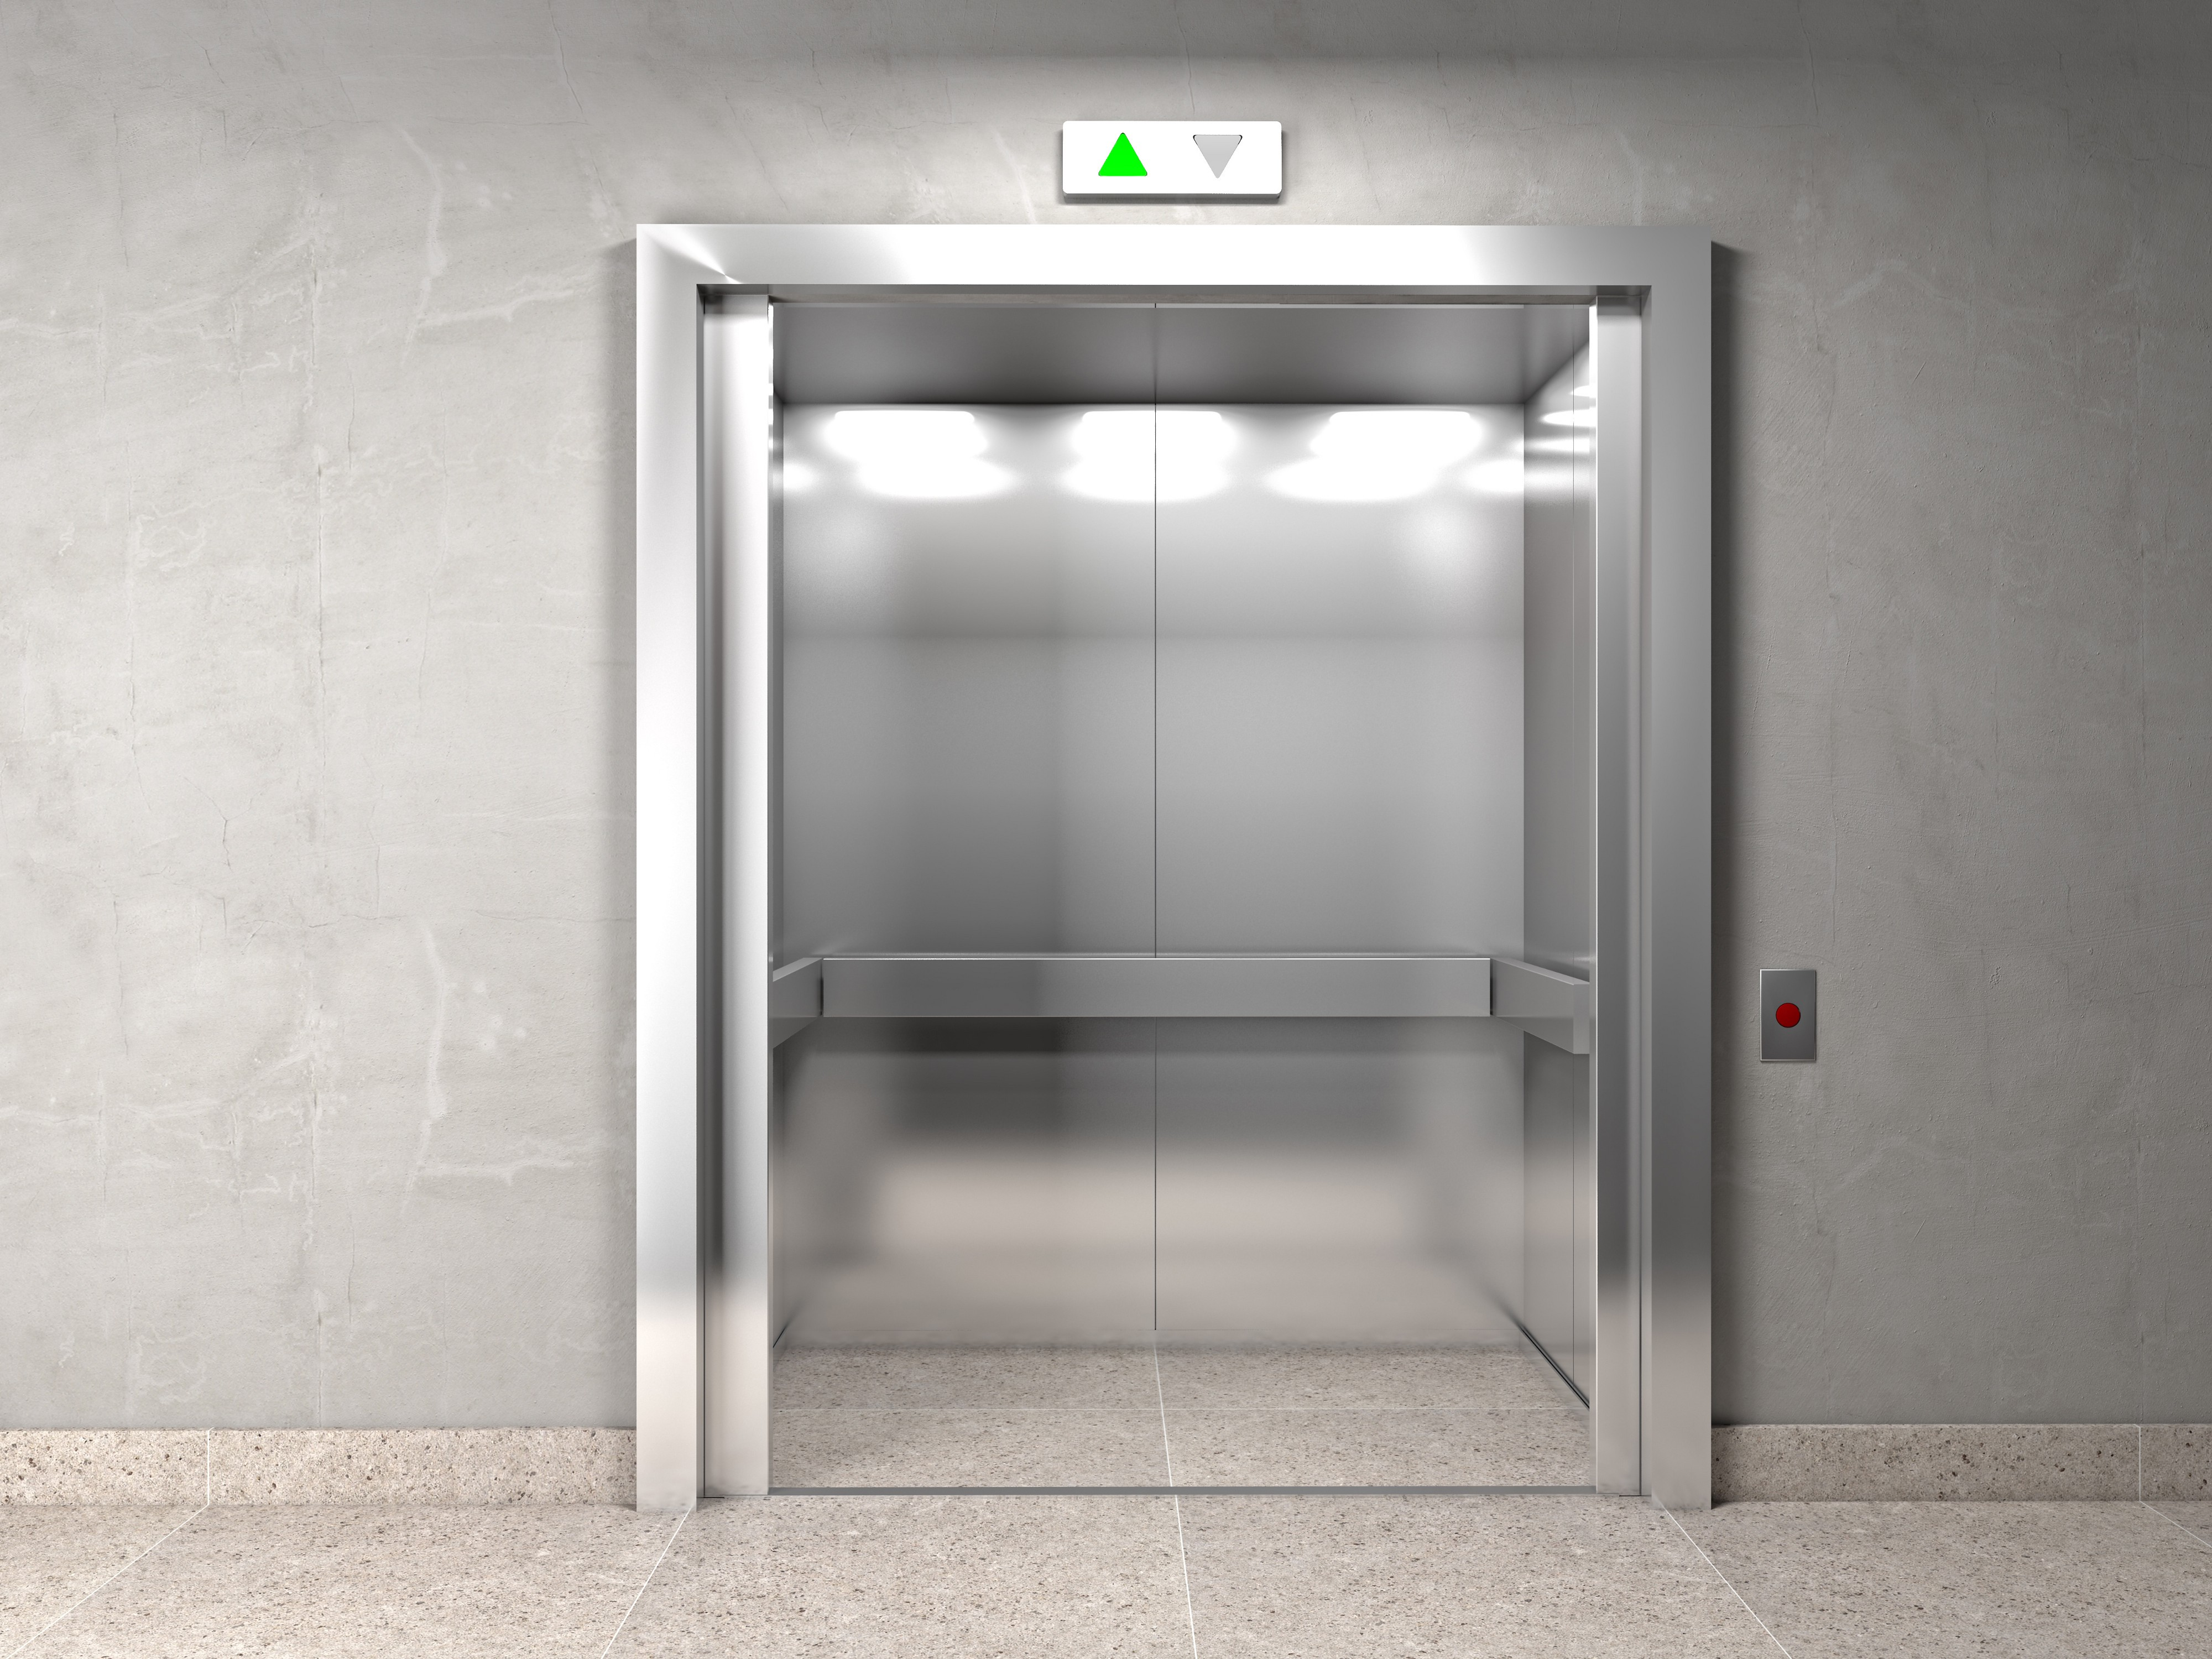
\includegraphics[width=\textwidth]{images/01_introduction/elevator.jpg}
    \end{column}\begin{column}{0.3\textwidth}
        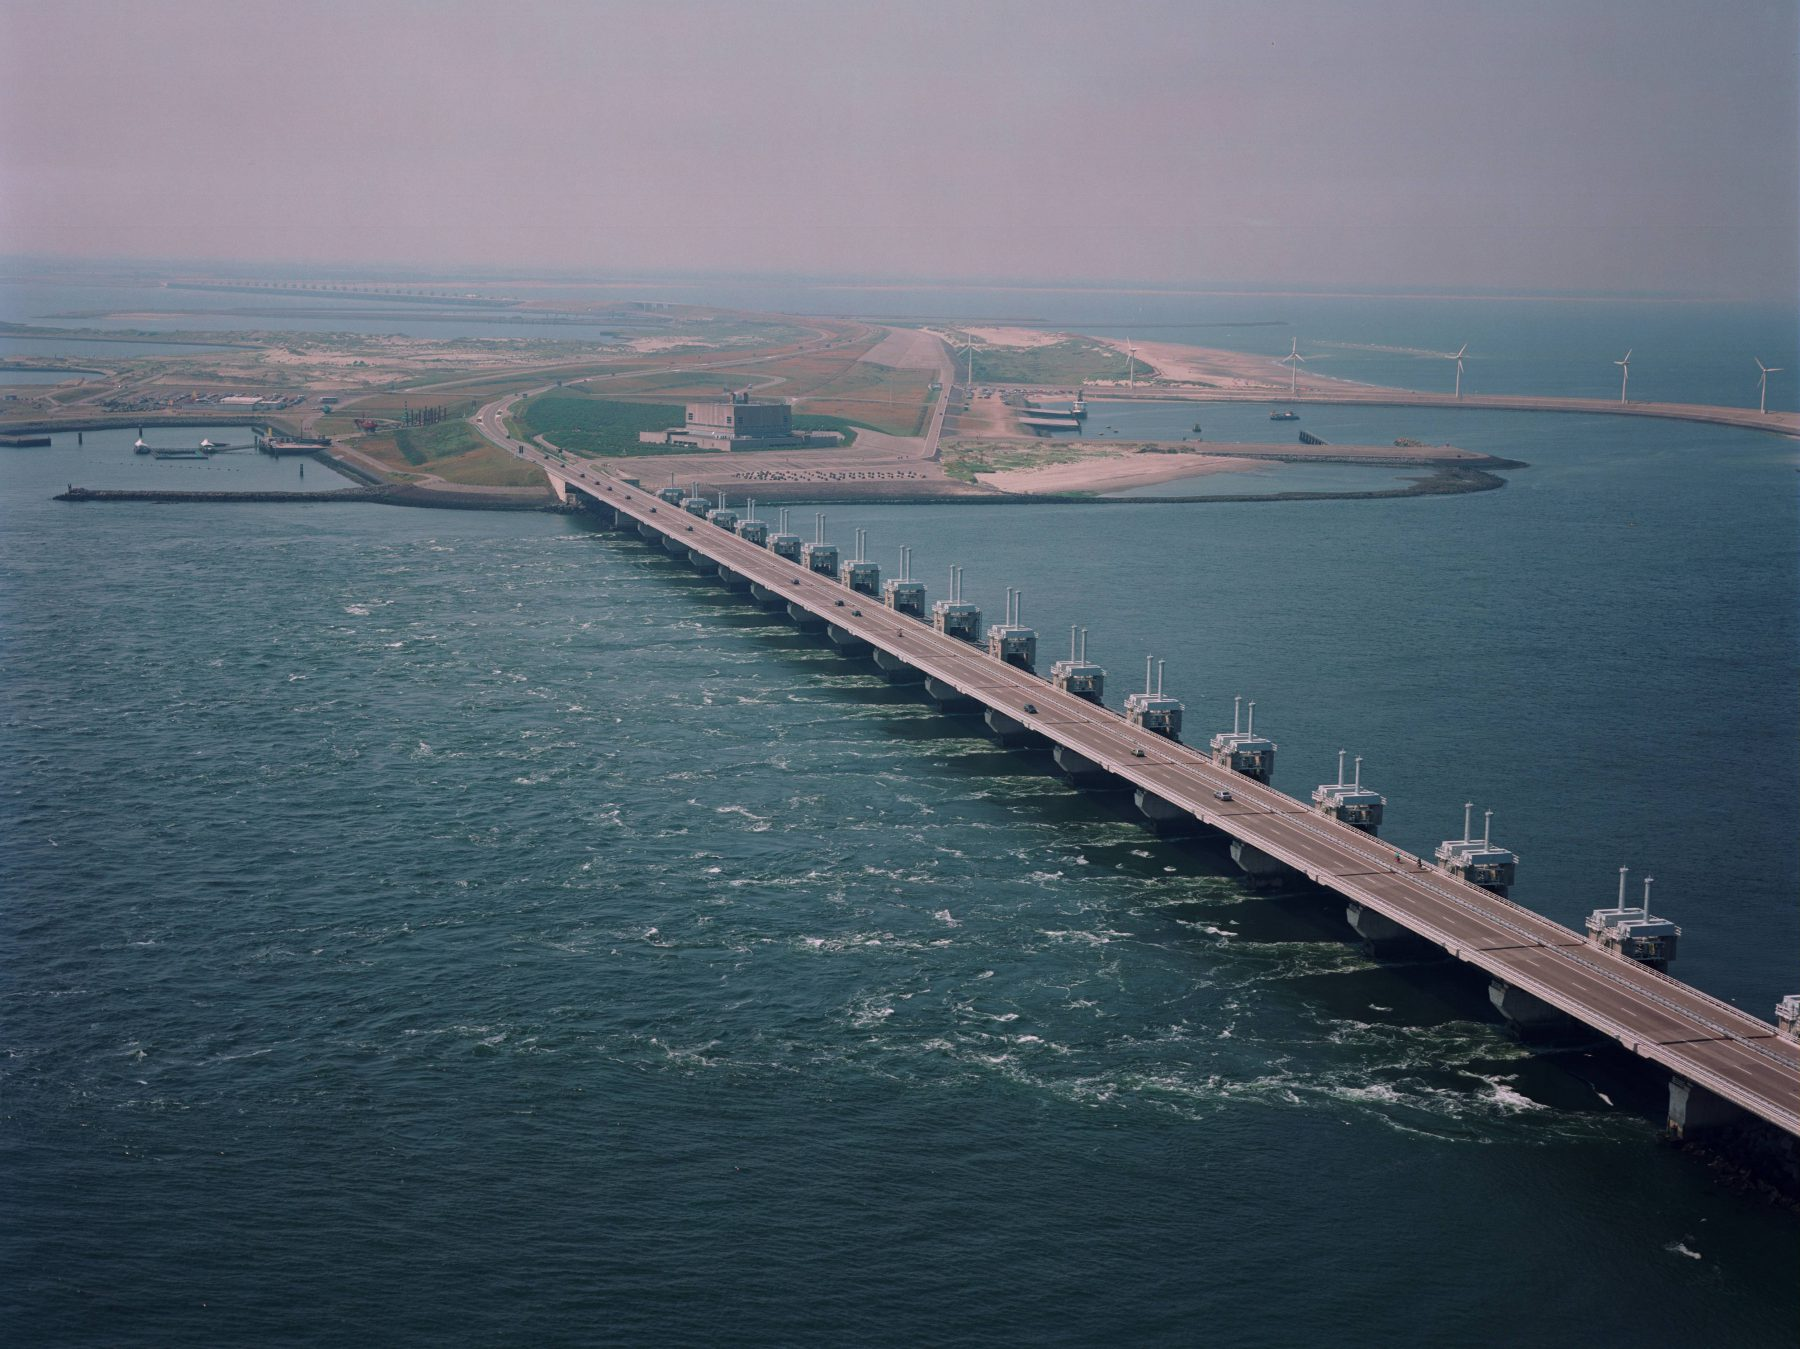
\includegraphics[width=\textwidth]{images/01_introduction/oosterscheldekering.jpg}
    \end{column}
\end{columns} 
\end{frame}

\note{
	\begin{itemize}
	    \item What have these 3 images in common?
	    \item They all make use of software systems that are crucial to be error free
	    \item How to ensure that software is error-free? Through software verification.
	\end{itemize}
}

\begin{frame}{Software verification through models}
    \centering
    \begin{tikzpicture} 
    \path
    (-3,1.5) node[inner sep=0pt](model) {% To use this figure in your LaTeX document
% import the package groove/resources/groove2tikz.sty
%
\begin{tikzpicture}[scale=0.6, every node/.style={scale=0.3}, name prefix=type-]
\node[type_node] (n0) at (0.560, -0.290) {\ml{\textbf{House}\\name: \textbf{string}}};
\node[type_node] (n1) at (0.600, -1.430) {\ml{\textbf{Room}\\number: \textbf{int}}};
\node[type_node] (n2) at (2.470, -1.435) {\ml{\textbf{Renter}}};
\node[type_node] (n3) at (2.470, -2.175) {\ml{\textit{\textbf{PaymentInterval}}}};
\node[type_node] (n4) at (1.070, -2.785) {\ml{\textbf{PaymentInterval\$MONTH}}};
\node[type_node] (n5) at (3.430, -2.785) {\ml{\textbf{PaymentInterval\$QUARTER}}};
\node[type_node] (n6) at (2.470, -0.375) {\ml{\textit{\textbf{Person}}\\age: \textbf{int}\\name: \textbf{string}}};

\path[subtype_edge](n2.north -| 2.470, -0.375) --  (n6) ;
\path[subtype_edge] (n4)  --  (n3) ;
\path[subtype_edge] (n5)  --  (n3) ;
\path[basic_edge](n2.west |- 0.600, -1.430) -- node[lab] {\ml{rents}} (n1) ;
\path[basic_edge, composite](n0.south -| 0.600, -1.430) -- node[lab] {\ml{rooms}} (n1) ;
\path[basic_edge](n2.south -| 2.470, -2.175) -- node[lab] {\ml{payment\_interval}} (n3) ;
\path[basic_edge](n1.east |- 2.470, -1.435) -- node[lab] {\ml{renter}} (n2) ;
\end{tikzpicture}
}
    (-3,-1.5) node[inner sep=0pt](checklist) {
\includegraphics[width=1.5cm]{images/01_introduction/checklist.pdf}}
    (0,0) node[inner sep=0pt](app) {
\includegraphics[width=2cm]{images/01_introduction/application.pdf}}
    (3,1.5) node[inner sep=0pt](correct) {\fontsize{40}{48} \selectfont \textcolor{ForestGreen}{\checkmark}}
    (3,-1.5) node[inner sep=0pt](incorrect) {\fontsize{40}{48} \selectfont \textcolor{red}{\ding{53}}};
    
    \path[]		
    (model) [-{Latex[width=10]}, black] edge node[above] {} (app)
    (checklist) [-{Latex[width=10]}, black] edge node[above] {} (app)
    (app) [-{Latex[width=10]}, black] edge node[above] {} (correct)
    (app) [-{Latex[width=10]}, black] edge node[above] {} (incorrect)
    ;
    \end{tikzpicture}
\end{frame}

\note{
    Explain the automated verification using a tool
	\begin{itemize}
	    \item Software model and the requirements that should be checked are given to verification software.
	    \item Verification software checks these requirements on the model.
	    \item It produces a result.
	\end{itemize}
	I will focus on obtaining the models that can be used for verification.
}

\begin{frame}{Software verification through models}
    \centering
    \begin{tikzpicture} 
    \path
    (-8,1.5) node[inner sep=0pt](fstmodel) {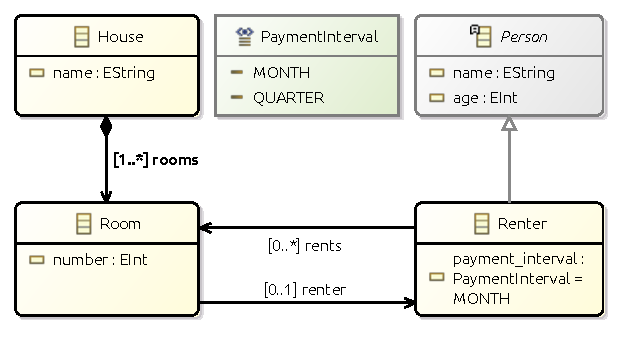
\includegraphics[width=3cm]{images/01_introduction/fstmodel.pdf}}
    (-3,1.5) node[inner sep=0pt](model) {% To use this figure in your LaTeX document
% import the package groove/resources/groove2tikz.sty
%
\begin{tikzpicture}[scale=0.6, every node/.style={scale=0.3}, name prefix=type-]
\node[type_node] (n0) at (0.560, -0.290) {\ml{\textbf{House}\\name: \textbf{string}}};
\node[type_node] (n1) at (0.600, -1.430) {\ml{\textbf{Room}\\number: \textbf{int}}};
\node[type_node] (n2) at (2.470, -1.435) {\ml{\textbf{Renter}}};
\node[type_node] (n3) at (2.470, -2.175) {\ml{\textit{\textbf{PaymentInterval}}}};
\node[type_node] (n4) at (1.070, -2.785) {\ml{\textbf{PaymentInterval\$MONTH}}};
\node[type_node] (n5) at (3.430, -2.785) {\ml{\textbf{PaymentInterval\$QUARTER}}};
\node[type_node] (n6) at (2.470, -0.375) {\ml{\textit{\textbf{Person}}\\age: \textbf{int}\\name: \textbf{string}}};

\path[subtype_edge](n2.north -| 2.470, -0.375) --  (n6) ;
\path[subtype_edge] (n4)  --  (n3) ;
\path[subtype_edge] (n5)  --  (n3) ;
\path[basic_edge](n2.west |- 0.600, -1.430) -- node[lab] {\ml{rents}} (n1) ;
\path[basic_edge, composite](n0.south -| 0.600, -1.430) -- node[lab] {\ml{rooms}} (n1) ;
\path[basic_edge](n2.south -| 2.470, -2.175) -- node[lab] {\ml{payment\_interval}} (n3) ;
\path[basic_edge](n1.east |- 2.470, -1.435) -- node[lab] {\ml{renter}} (n2) ;
\end{tikzpicture}
}
    (-3,-1.5) node[inner sep=0pt](checklist) {
\includegraphics[width=1.5cm]{images/01_introduction/checklist.pdf}}
    (0,0) node[inner sep=0pt](app) {
\includegraphics[width=2cm]{images/01_introduction/application.pdf}}
    (3,1.5) node[inner sep=0pt](correct) {\fontsize{40}{48} \selectfont \textcolor{ForestGreen}{\checkmark}}
    (3,-1.5) node[inner sep=0pt](incorrect) {\fontsize{40}{48} \selectfont \textcolor{red}{\ding{53}}};
    
    \path[]
    (fstmodel) [-{Latex[width=10]}, black] edge node[above] {Transform} (model)
    (model) [-{Latex[width=10]}, black] edge node[above] {} (app)
    (checklist) [-{Latex[width=10]}, black] edge node[above] {} (app)
    (app) [-{Latex[width=10]}, black] edge node[above] {} (correct)
    (app) [-{Latex[width=10]}, black] edge node[above] {} (incorrect)
    ;
    \end{tikzpicture}
\end{frame}

\begin{frame}{Model transformations}
    \begin{itemize}
        \item Concept from Model-driven engineering (MDE)
        \item Use a systematic approach to transform models within/between modelling languages
        \item For use in software verification, a formal foundation is required.
    \end{itemize}
\end{frame}

\note{
	\begin{itemize}
	    \item Explain that transforming models is a concept borrowed from MDE.
	    \item Explain that for verification, we want the model transformations to be proven correct, however, in most implementations this is not the case.
	\end{itemize}
}

\begin{frame}{Scope}
    \begin{itemize}
        \item Model transformations between
        \begin{itemize}
            \item EMF/Ecore
            \item GROOVE graphs
        \end{itemize}
        \item Only syntactical correctness is proven
    \end{itemize}
\end{frame}

\note{
	\begin{itemize}
	    \item Explain that my thesis focuses on solely 2 languages.
	    \item Explain that only syntactical correctness is considered within this work. Sematics are left for future work.
	\end{itemize}
}

\begin{frame}{Research questions}
    What is a suitable formalisation for composable model transformations between Ecore and GROOVE that gives rise to correct model transformations between Ecore and GROOVE?
    \pause
    \begin{itemize}
        \item What is a suitable formalisation of Ecore models and what Ecore models are valid within this formalisation? 
        \item What is a suitable formalisation of GROOVE grammars and what GROOVE grammars are valid within this formalisation? 
        \pause
        \item What is a suitable formalisation for the model transformations between Ecore and GROOVE?
        \item What model transformations are correct within the formalisation?
        \pause
        \item How can correct model transformations between Ecore and GROOVE be composed?
    \end{itemize}
\end{frame}

\note{
	\begin{itemize}
	    \item Explain the main research question. We already discussed the ingredients of the problem, so we can use that.
	    \begin{itemize}
	        \item The first two subquestions discuss the formal descriptions of EMF/Ecore and GROOVE.
	        \item The third subquestion discusses the formal description of the model transformations.
	        \item The fourth question discusses the correctness properties.
	        \item The last question is about composability, see below.
	    \end{itemize}
	    \item Leave composability on a cliffhanger. This is the only detail that was not discussed yet. In order to explain this in detail, we should first see why composability is a nice property to have, which is discussed as part of the next section.
	\end{itemize}
}

\begin{frame}{Validation}
    \begin{itemize}
        \item All proofs are checked using Isabelle, a theorem prover.
        \item Example applications show the feasibility and existance of correct model transformations.
    \end{itemize}
\end{frame}

\note{
	\begin{itemize}
	    \item The work contains a lot of mathematical formalisations and proofs, validating these is done through Isabelle, a proof assistant.
	    \item Explain that a formalisation is useless if no correct model transformations exist. An application of the proven theory shows that this is not the case.
	\end{itemize}
}

\begin{frame}{Contribution}
    Existing work on the formalisation of model transformations exists. Most important work is in the area of Triple Graph Grammars.\\
    \pause
    \vspace{0.5cm}
    What is the contribution of this thesis?
    \begin{itemize}
        \item Different approach, no conversion to graphs
        \item First formalisation of transformations between Ecore \& GROOVE specifically
    \end{itemize}
\end{frame}

\note{
	\begin{itemize}
	    \item Explain that there is earlier work on the formalisation of model transformations. Most important work is in the area of TGGs, which use graph formalisations for the modelling languages.
	    \item Explain the contribution of this work, which does not use triple graph grammars, which is an entirely different approach.
	    \item Moreover, this work focuses on Ecore/GROOVE transformations specifically, which gives rise to an formalisation that is concrete considering existing work.
	\end{itemize}
}

\begin{frame}{Contents}
\tableofcontents
\end{frame}
\section{Modelling languages}

\begin{frame}{Modelling languages}
    ``A modelling language is any artificial language that can be used to express systems in a structure that is defined by a consistent set of rules.''
\end{frame}

\begin{frame}{Modelling languages}
\begin{columns}[c]
    \begin{column}{0.05\textwidth}
    \end{column}\begin{column}{0.45\textwidth}
        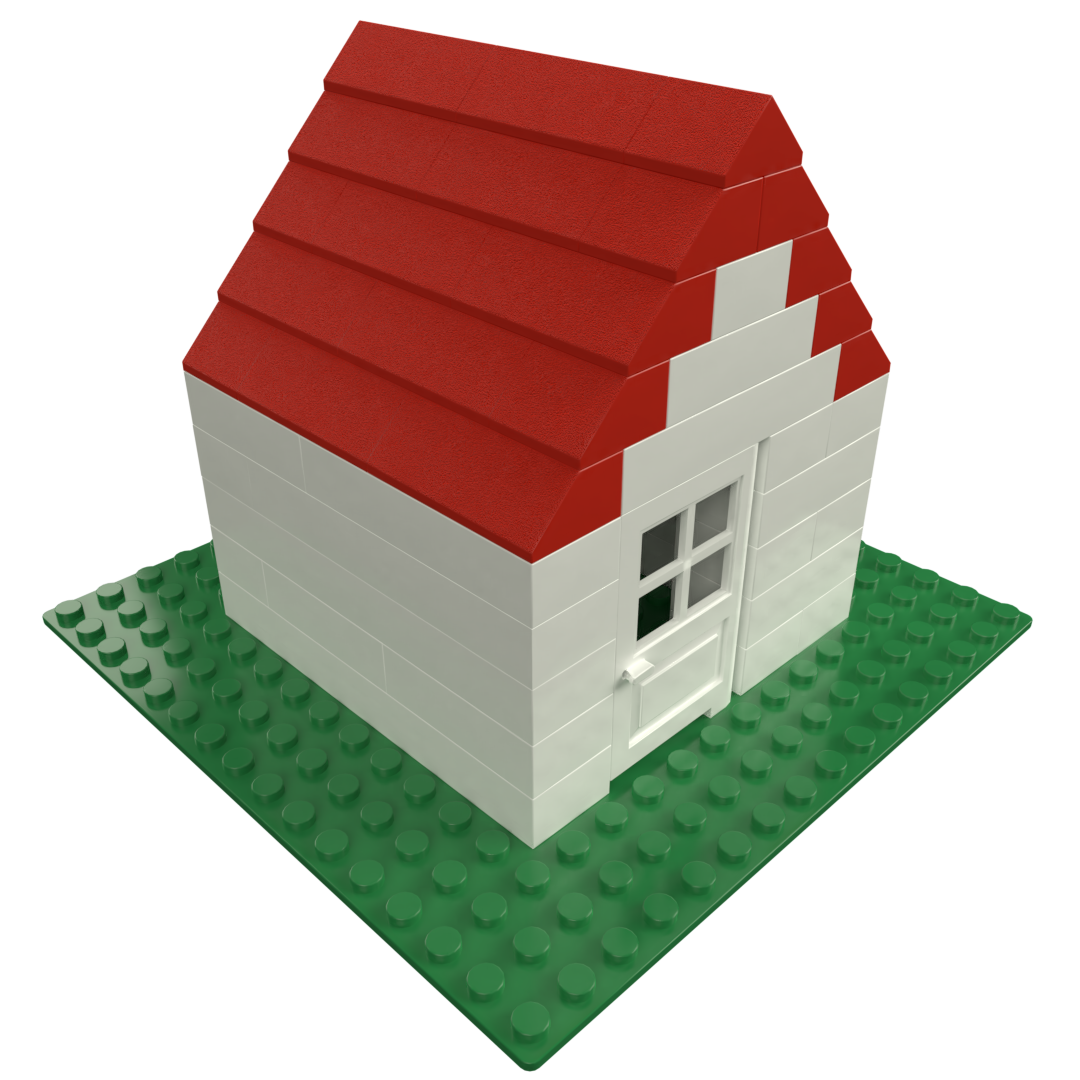
\includegraphics[width=\textwidth]{images/02_modelling_languages/lego_house.png}
    \end{column}\begin{column}{0.4\textwidth}
        \centering
        
\includegraphics[width=0.5\textwidth]{images/02_modelling_languages/LEGO_logo.pdf}
        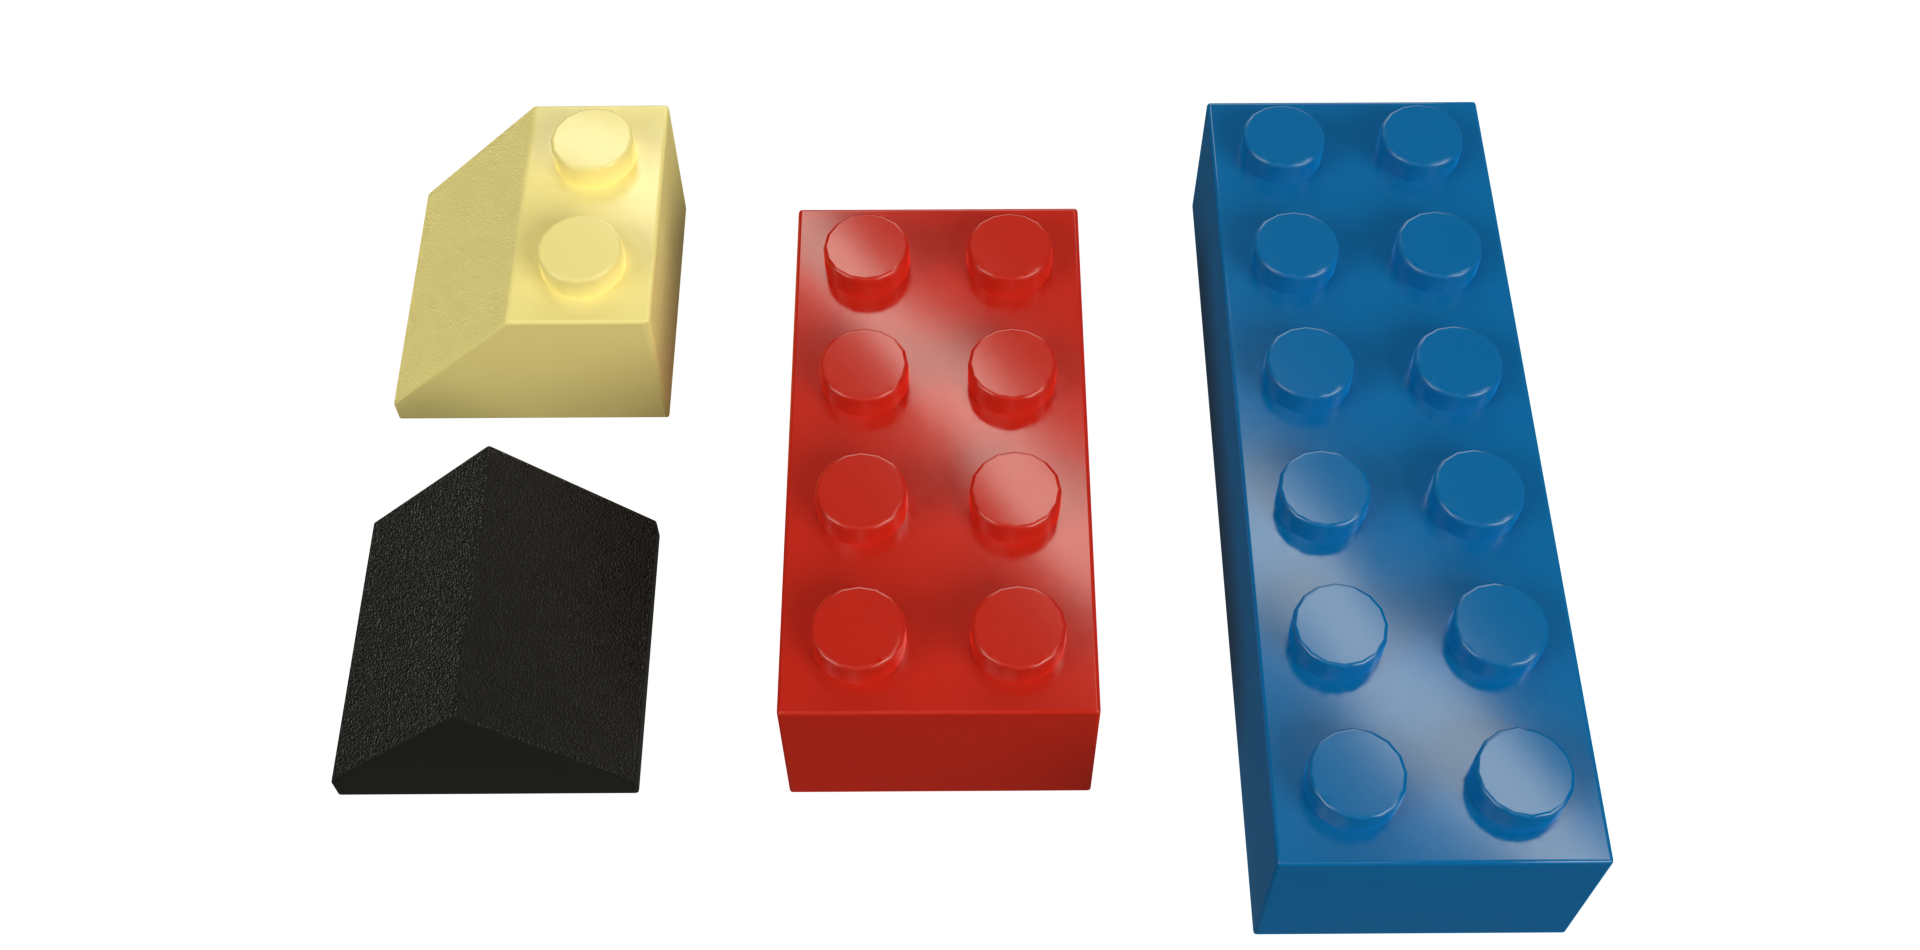
\includegraphics[width=\textwidth]{images/02_modelling_languages/lego_brick_examples.png}
    \end{column}
\end{columns}
\end{frame}

\note{
	\begin{itemize}
	    \item Explain what a modelling language is informally, ignore the definition.
	    \item Explain that you could think of Lego as a modelling language.
	\end{itemize}
}

\begin{frame}{Modelling languages}
    EMF/Ecore
    \begin{itemize}
        \item Eclipse Modelling Framework
        \item Modelling framework and code generation facility
        \item Modelling language rules enforced by metamodel Ecore
    \end{itemize}
    \pause
    GROOVE
    \begin{itemize}
        \item GRaphs for Object-Oriented VErification
        \item Software verification tool using graph grammars
        \item Modelling language rules based on graph grammars
    \end{itemize}
\end{frame}

\note{
	\begin{itemize}
	    \item Explain that within this thesis, we use software modelling languages.
	    \item Explain shortly what Ecore is
	    \item Explain shortly what GROOVE is
	\end{itemize}
}

\begin{frame}{Modelling languages}
    For Ecore, 2 different model types are considered:
    \begin{itemize}
        \item Type models, directly based on the Ecore metamodel
        \item Instance models, based on a type model
    \end{itemize}
    \pause
    For GROOVE, 2 different graph types are considered:
    \begin{itemize}
        \item Type graphs
        \item Instance graphs, based on a type graph
    \end{itemize}
\end{frame}

\note{
	\begin{itemize}
	    \item Explain that for Ecore, two different levels of models are considered, type models and instance models.
	    \begin{itemize}
	        \item Type models are best viewed as UML class diagrams
	        \item Instance models are instatiations of these diagrams.
	    \end{itemize}
	    \item Explain that for GROOVE, we have similar levels
	    \begin{itemize}
	        \item Type models will be transformed into type graphs, which are graphs that define a some structure of node types and edge types.
	        \item Instance models are transformed into instance graphs, which is an instantiation of the structure defined by the type graph.
	    \end{itemize}
	\end{itemize}
}

\begin{frame}{Ecore type model}
    \centering
    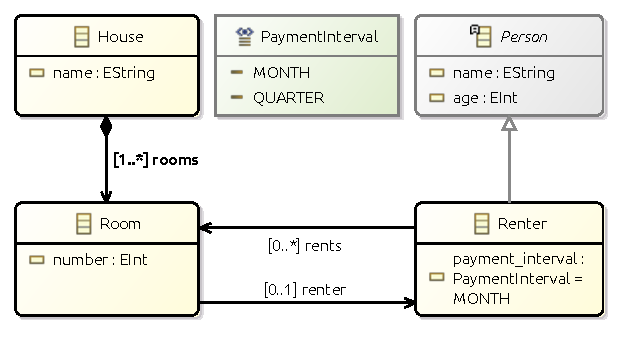
\includegraphics[width=0.9\textwidth,trim={0 0.45cm 0 0.25cm},clip]{images/02_modelling_languages/type_model_example.pdf}
\end{frame}

\begin{frame}{GROOVE type graph}
    \centering
    % To use this figure in your LaTeX document
% import the package groove/resources/groove2tikz.sty
%
\begin{tikzpicture}[scale=\tikzscale,name prefix=type-]
\node[type_node] (n0) at (0.560, -0.290) {\ml{\textbf{House}\\name: \textbf{string}}};
\node[type_node] (n1) at (0.600, -1.430) {\ml{\textbf{Room}\\number: \textbf{int}}};
\node[type_node] (n2) at (2.470, -1.435) {\ml{\textbf{Renter}}};
\node[type_node] (n3) at (2.470, -2.175) {\ml{\textit{\textbf{PaymentInterval}}}};
\node[type_node] (n4) at (1.170, -2.785) {\ml{\textbf{PaymentInterval\$MONTH}}};
\node[type_node] (n5) at (3.830, -2.785) {\ml{\textbf{PaymentInterval\$QUARTER}}};
\node[type_node] (n6) at (2.470, -0.375) {\ml{\textit{\textbf{Person}}\\age: \textbf{int}\\name: \textbf{string}}};

\path[subtype_edge](n2.north -| 2.470, -0.375) --  (n6) ;
\path[subtype_edge] (n4)  --  (n3) ;
\path[subtype_edge] (n5)  --  (n3) ;
\path[basic_edge](n2.west |- 0.600, -1.430) -- node[lab] {\ml{rents}} (n1) ;
\path[basic_edge, composite](n0.south -| 0.600, -1.430) -- node[lab] {\ml{rooms}} (n1) ;
\path[basic_edge](n2.south -| 2.470, -2.175) -- node[lab] {\ml{payment\_interval}} (n3) ;
\path[basic_edge](n1.east |- 2.470, -1.435) -- node[lab] {\ml{renter}} (n2) ;
\end{tikzpicture}

\end{frame}

\note{
	\begin{itemize}
	    \item Explain type model and type graph. Show that they have the same elements.
	    \item Explain that certain elements need to be encoded.
	\end{itemize}
}

\begin{frame}{Ecore instance model}
    \centering
    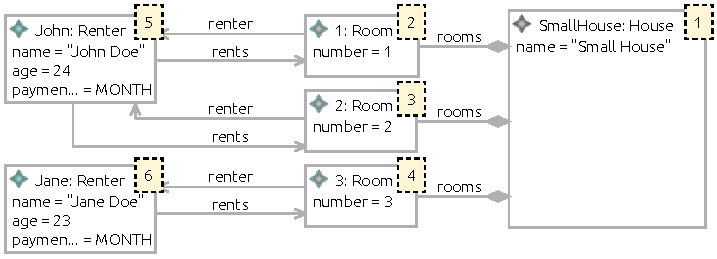
\includegraphics[]{images/02_modelling_languages/instance_model_example.pdf}
\end{frame}

\begin{frame}{GROOVE instance graph}
    \centering
    % To use this figure in your LaTeX document
% import the package groove/resources/groove2tikz.sty
%
\begin{tikzpicture}[scale=\tikzscale,name prefix=start-]
\node[basic_node] (n0) at (2.235, -0.335) {\ml{\uline{\textit{Renter1}} : \textbf{Renter}\\age = 24\\name = "J.A."}};
\node[basic_node] (n1) at (2.225, -2.305) {\ml{\uline{\textit{Renter2}} : \textbf{Renter}\\age = 23\\name = "M.S."}};
\node[basic_node] (n2) at (1.005, -1.345) {\ml{\textbf{PaymentInterval\$MONTH}}};
\node[basic_node] (n3) at (4.605, -0.330) {\ml{\uline{\textit{Longhorn}} : \textbf{Room}\\number = 1}};
\node[basic_node] (n4) at (4.585, -1.370) {\ml{\uline{\textit{Shorthorn}} : \textbf{Room}\\number = 2}};
\node[basic_node] (n5) at (4.595, -2.330) {\ml{\uline{\textit{onghornLay}} : \textbf{Room}\\number = 3}};
\node[basic_node] (n6) at (6.975, -1.380) {\ml{\uline{\textit{TwoRem}} : \textbf{House}\\name = "Small House"}};

\path[basic_edge] (n6)  -- node[lab] {\ml{rooms}} (n5) ;
\path[basic_edge](n6.west |- 4.585, -1.370) -- node[lab] {\ml{rooms}} (n4) ;
\path[basic_edge](n3.west |- 2.235, -0.235) -- node[lab] {\ml{renter}} (n0) ;
\path[basic_edge] (n4.west)  -- node[lab] {\ml{renter}} (n0) ;
\path[basic_edge](n5.west |- 2.225, -2.205) -- node[lab] {\ml{renter}} (n1) ;
\path[basic_edge] (n0)  -- node[lab] {\ml{payment\_interval}} (n2) ;
\path[basic_edge] (n6)  -- node[lab] {\ml{rooms}} (n3) ;
\path[basic_edge] (n0) -- node[lab] {\ml{rents}} (n3.west |- 4.605, -0.430) ;
\path[basic_edge] (n1)  -- node[lab] {\ml{payment\_interval}} (n2) ;
\path[basic_edge](n1) -- node[lab] {\ml{rents}} (n5.west |- 4.595, -2.430) ;
\path[basic_edge] (n0)  -- node[lab] {\ml{rents}} (n4.north) ;
\end{tikzpicture}

\end{frame}

\note{
	\begin{itemize}
	    \item Explain instance model and instance graph. Show that it are instantiations of their type counterparts.
	\end{itemize}
}
\section{Transformation framework}

\begin{frame}{How to transform this type model...}
    \centering
    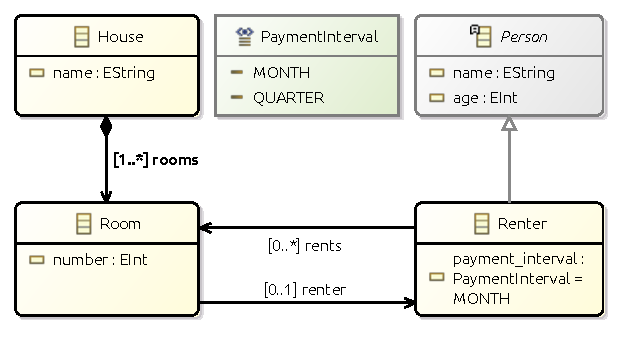
\includegraphics[trim={0 0.45cm 0 0.25cm},clip]{images/02_modelling_languages/type_model_example.pdf}
\end{frame}

\begin{frame}{...into this type graph}
    \centering
    % To use this figure in your LaTeX document
% import the package groove/resources/groove2tikz.sty
%
\begin{tikzpicture}[scale=\tikzscale,name prefix=type-]
\node[type_node] (n0) at (0.560, -0.290) {\ml{\textbf{House}\\name: \textbf{string}}};
\node[type_node] (n1) at (0.600, -1.430) {\ml{\textbf{Room}\\number: \textbf{int}}};
\node[type_node] (n2) at (2.470, -1.435) {\ml{\textbf{Renter}}};
\node[type_node] (n3) at (2.470, -2.175) {\ml{\textit{\textbf{PaymentInterval}}}};
\node[type_node] (n4) at (1.170, -2.785) {\ml{\textbf{PaymentInterval\$MONTH}}};
\node[type_node] (n5) at (3.830, -2.785) {\ml{\textbf{PaymentInterval\$QUARTER}}};
\node[type_node] (n6) at (2.470, -0.375) {\ml{\textit{\textbf{Person}}\\age: \textbf{int}\\name: \textbf{string}}};

\path[subtype_edge](n2.north -| 2.470, -0.375) --  (n6) ;
\path[subtype_edge] (n4)  --  (n3) ;
\path[subtype_edge] (n5)  --  (n3) ;
\path[basic_edge](n2.west |- 0.600, -1.430) -- node[lab] {\ml{rents}} (n1) ;
\path[basic_edge, composite](n0.south -| 0.600, -1.430) -- node[lab] {\ml{rooms}} (n1) ;
\path[basic_edge](n2.south -| 2.470, -2.175) -- node[lab] {\ml{payment\_interval}} (n3) ;
\path[basic_edge](n1.east |- 2.470, -1.435) -- node[lab] {\ml{renter}} (n2) ;
\end{tikzpicture}

\end{frame}

\begin{frame}{And what about transforming this instance model...}
    \centering
    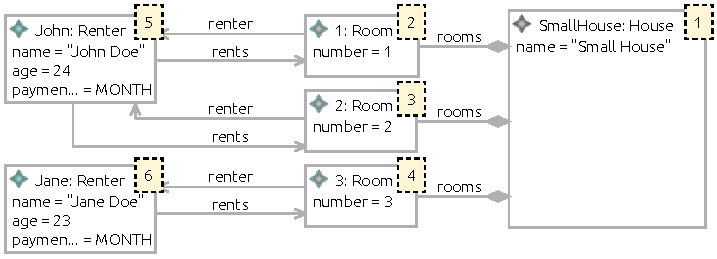
\includegraphics[]{images/02_modelling_languages/instance_model_example.pdf}
\end{frame}

\begin{frame}{...into this instance graph}
    \centering
    % To use this figure in your LaTeX document
% import the package groove/resources/groove2tikz.sty
%
\begin{tikzpicture}[scale=\tikzscale,name prefix=start-]
\node[basic_node] (n0) at (2.235, -0.335) {\ml{\uline{\textit{Renter1}} : \textbf{Renter}\\age = 24\\name = "J.A."}};
\node[basic_node] (n1) at (2.225, -2.305) {\ml{\uline{\textit{Renter2}} : \textbf{Renter}\\age = 23\\name = "M.S."}};
\node[basic_node] (n2) at (1.005, -1.345) {\ml{\textbf{PaymentInterval\$MONTH}}};
\node[basic_node] (n3) at (4.605, -0.330) {\ml{\uline{\textit{Longhorn}} : \textbf{Room}\\number = 1}};
\node[basic_node] (n4) at (4.585, -1.370) {\ml{\uline{\textit{Shorthorn}} : \textbf{Room}\\number = 2}};
\node[basic_node] (n5) at (4.595, -2.330) {\ml{\uline{\textit{onghornLay}} : \textbf{Room}\\number = 3}};
\node[basic_node] (n6) at (6.975, -1.380) {\ml{\uline{\textit{TwoRem}} : \textbf{House}\\name = "Small House"}};

\path[basic_edge] (n6)  -- node[lab] {\ml{rooms}} (n5) ;
\path[basic_edge](n6.west |- 4.585, -1.370) -- node[lab] {\ml{rooms}} (n4) ;
\path[basic_edge](n3.west |- 2.235, -0.235) -- node[lab] {\ml{renter}} (n0) ;
\path[basic_edge] (n4.west)  -- node[lab] {\ml{renter}} (n0) ;
\path[basic_edge](n5.west |- 2.225, -2.205) -- node[lab] {\ml{renter}} (n1) ;
\path[basic_edge] (n0)  -- node[lab] {\ml{payment\_interval}} (n2) ;
\path[basic_edge] (n6)  -- node[lab] {\ml{rooms}} (n3) ;
\path[basic_edge] (n0) -- node[lab] {\ml{rents}} (n3.west |- 4.605, -0.430) ;
\path[basic_edge] (n1)  -- node[lab] {\ml{payment\_interval}} (n2) ;
\path[basic_edge](n1) -- node[lab] {\ml{rents}} (n5.west |- 4.595, -2.430) ;
\path[basic_edge] (n0)  -- node[lab] {\ml{rents}} (n4.north) ;
\end{tikzpicture}

\end{frame}

\begin{frame}{Transformation framework}
    \begin{itemize}
        \item There exist infinitely many possible models and graphs.
        \item As a consequence, there are infinitely many possible model transformations.\pause
        \item Conclusion: It is not possible to separately proof all of them.
    \end{itemize}
    \vspace{1cm}
    How to solve this issue?
\end{frame}

\note{
	\begin{itemize}
	    \item Explain that the problem is not trivial, especially since correctness needs to be proven.
	    \item Explain that the approach is key, as it is impossible to have a proof for all possible model transformations.
	    \item Cliffhanger: How to solve the issue of infinitely many model transformations.
	\end{itemize}
}

\begin{frame}<1-2>[label=framework]{Transformation framework}
    What if transformations and their proofs can be composed? \pause
    \begin{itemize}
        \item The well-known concept of divide and conquer
        \item Use small additions to a model to create a larger model. \pause
        \item Give the 'small additions' a corresponding transformation.
        \item Apply small additions in both languages at the same time, create a larger model transformation with each step.
    \end{itemize}
\end{frame}

\begin{frame}{Combining models}
    The concept of building models out of small parts... \pause
    We have seen that before!
    \begin{columns}[c]
        \begin{column}{0.05\textwidth}
        \end{column}\begin{column}{0.35\textwidth}
            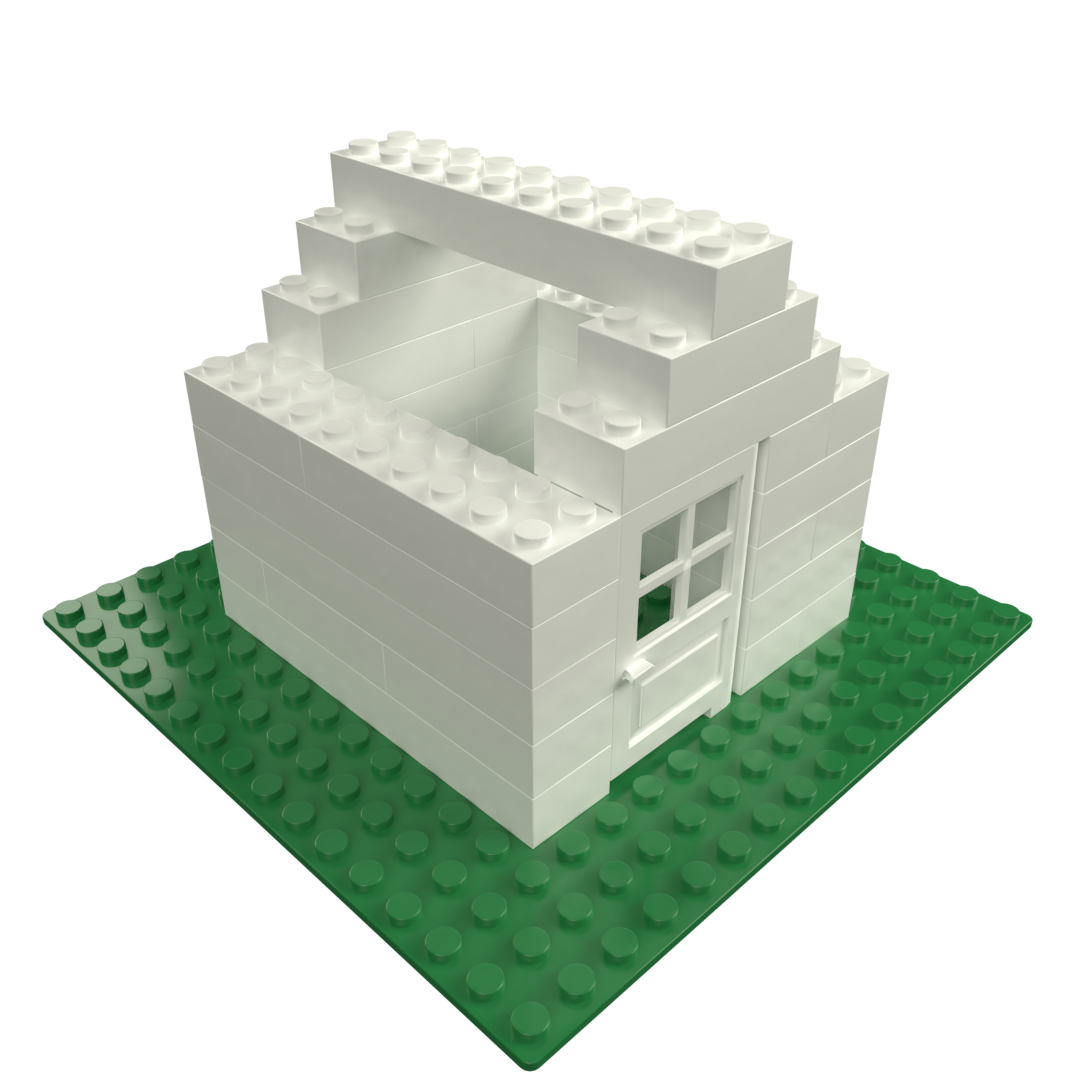
\includegraphics[width=\textwidth]{images/03_transformation_framework/lego_house_roofless.png}
        \end{column}\begin{column}{0.2\textwidth}
            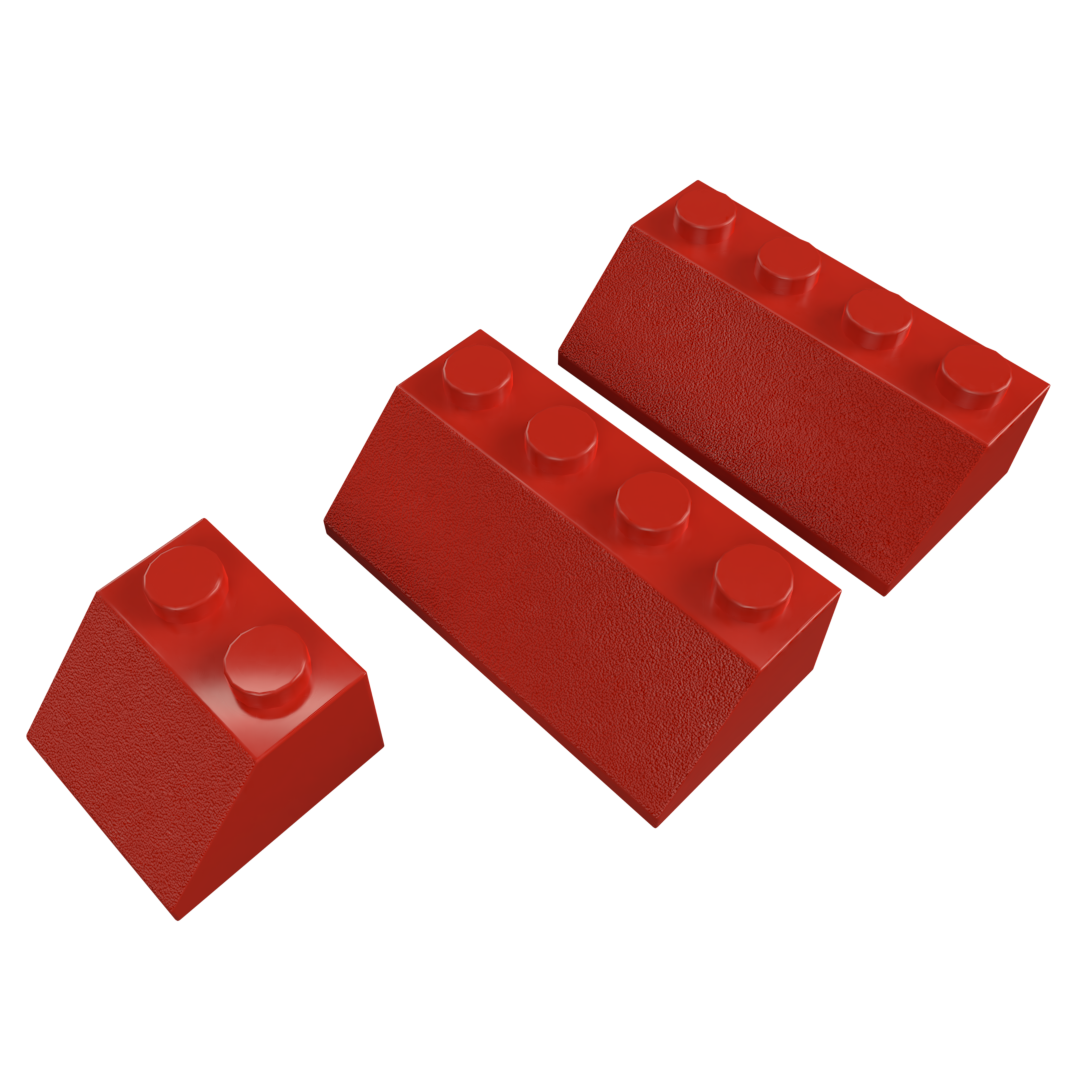
\includegraphics[width=\textwidth]{images/03_transformation_framework/lego_roof_pieces.png}
        \end{column}\begin{column}{0.35\textwidth}
            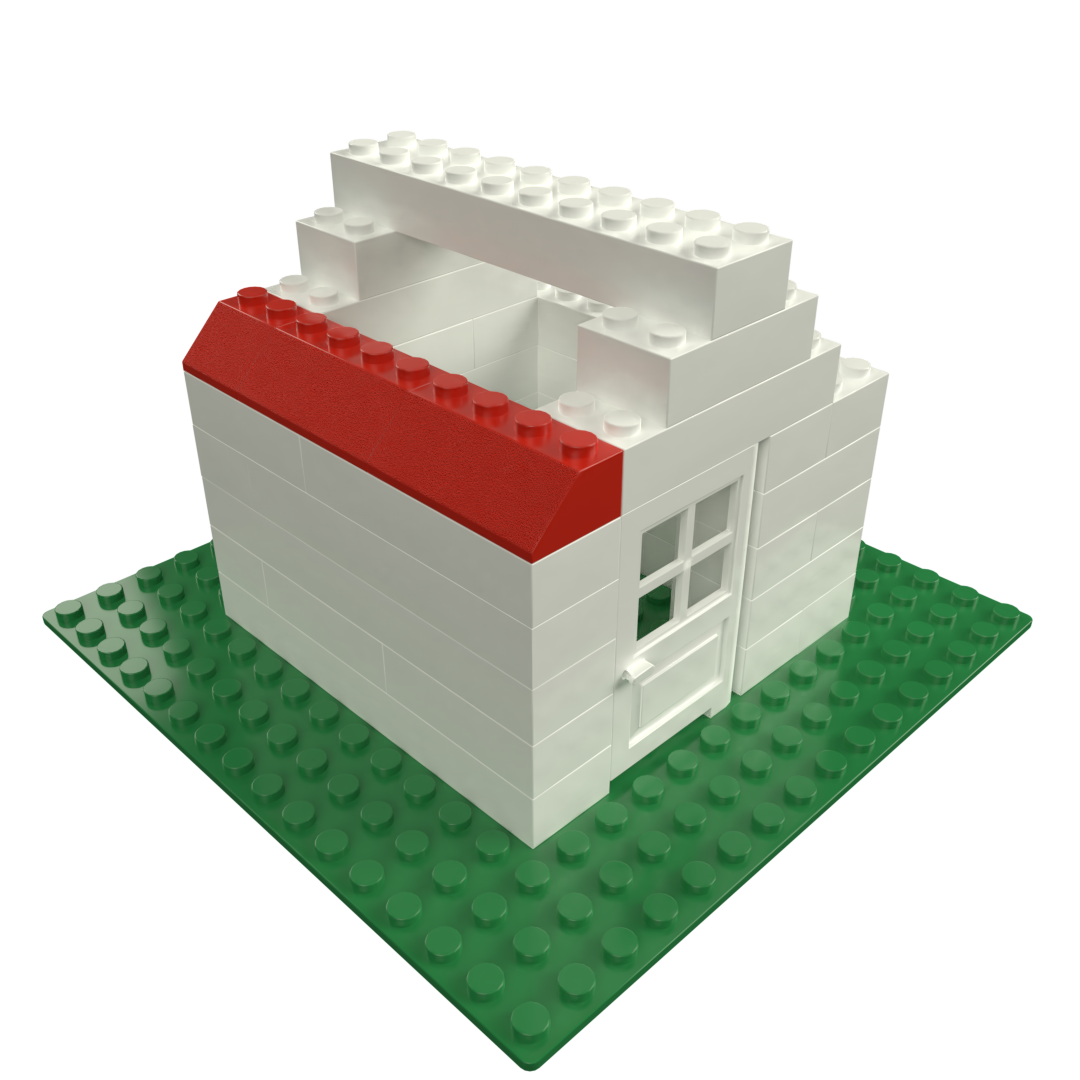
\includegraphics[width=\textwidth]{images/03_transformation_framework/lego_house_roof_step.png}
        \end{column}
    \end{columns} 
\end{frame}

\againframe<3>{framework}

\note{
	\begin{itemize}
	    \item Roughly explain that building the models iteratively is key.
	    \item This concept is also known from Lego!
	    \item These small steps are easier to create correctness proofs for.
	    \item Small steps can be combined over and over, as a way to create correct model transformations.
	\end{itemize}
}

\begin{frame}{Structure}
    \centering
    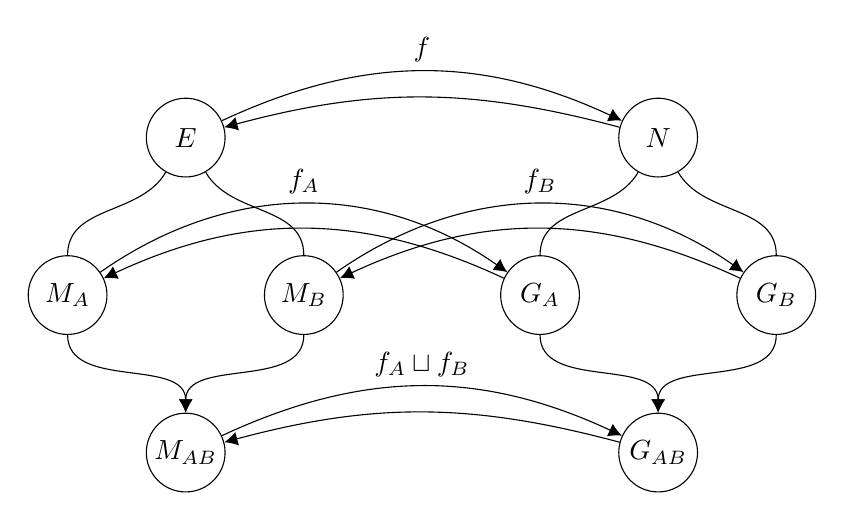
\begin{tikzpicture} 
    \path
    (-3,4) node[circle,draw,minimum size=10mm,inner sep=0pt](ME) {$E$}
    (-4.5,2) node[circle,draw,minimum size=10mm,inner sep=0pt](MA) {$M_A$}
    (-1.5,2) node[circle,draw,minimum size=10mm,inner sep=0pt](MB) {$M_B$}
    (-3,0) node[circle,draw,minimum size=10mm,inner sep=0pt](MAB) {$M_{AB}$}
    
    (3,4) node[circle,draw,minimum size=10mm,inner sep=0pt](GN) {$N$}
    (1.5,2) node[circle,draw,minimum size=10mm,inner sep=0pt](GA) {$G_A$}
    (4.5,2) node[circle,draw,minimum size=10mm,inner sep=0pt](GB) {$G_B$}
    (3,0) node[circle,draw,minimum size=10mm,inner sep=0pt](GAB) {$G_{AB}$};
    
    \path[]		
    (ME) [-, black, out=240, in=90] edge node[above] {} (MA)
    (ME) [-, black, out=300, in=90] edge node[above] {} (MB)
    
    (MA) [-{Latex[width=5]}, black, out=270, in=90] edge node[above] {} (MAB)
    (MB) [-{Latex[width=5]}, black, out=270, in=90] edge node[above] {} (MAB)
    
    (GN) [-, black, out=240, in=90] edge node[above] {} (GA)
    (GN) [-, black, out=300, in=90] edge node[above] {} (GB)
    
    (GA) [-{Latex[width=5]}, black, out=270, in=90] edge node[above] {} (GAB)
    (GB) [-{Latex[width=5]}, black, out=270, in=90] edge node[above] {} (GAB)
    
    (ME) [-{Latex[width=5]}, black, out=25, in=155] edge node[above] {$f$} (GN)
    (GN) [-{Latex[width=5]}, black, out=165, in=15] edge node[above] {} (ME)
    
    (MA) [-{Latex[width=5]}, black, out=35, in=145] edge node[above] {$f_A$} (GA)
    (GA) [-{Latex[width=5]}, black, out=155, in=25] edge node[above] {} (MA)
    
    (MB) [-{Latex[width=5]}, black, out=35, in=145] edge node[above] {$f_B$} (GB)
    (GB) [-{Latex[width=5]}, black, out=155, in=25] edge node[above] {} (MB)
    
    (MAB) [-{Latex[width=5]}, black, out=25, in=155] edge node[above] {$f_{A} \sqcup f_{B}$} (GAB)
    (GAB) [-{Latex[width=5]}, black, out=165, in=15] edge node[above] {} (MAB)
    ;
    \end{tikzpicture}
\end{frame}

\note{
	\begin{itemize}
	    \item Explain on an abstract level what the transformation framework is.
	    \item Make clear that when applying steps to the model side, a similar step is applied to the graph side.
	    \item Similar means, there is a correct transformation between the added steps.
	\end{itemize}
}

\begin{frame}{Combining transformations}
\begin{columns}[c]
    \begin{column}{0.05\textwidth}
    \end{column}\begin{column}{0.3\textwidth}
        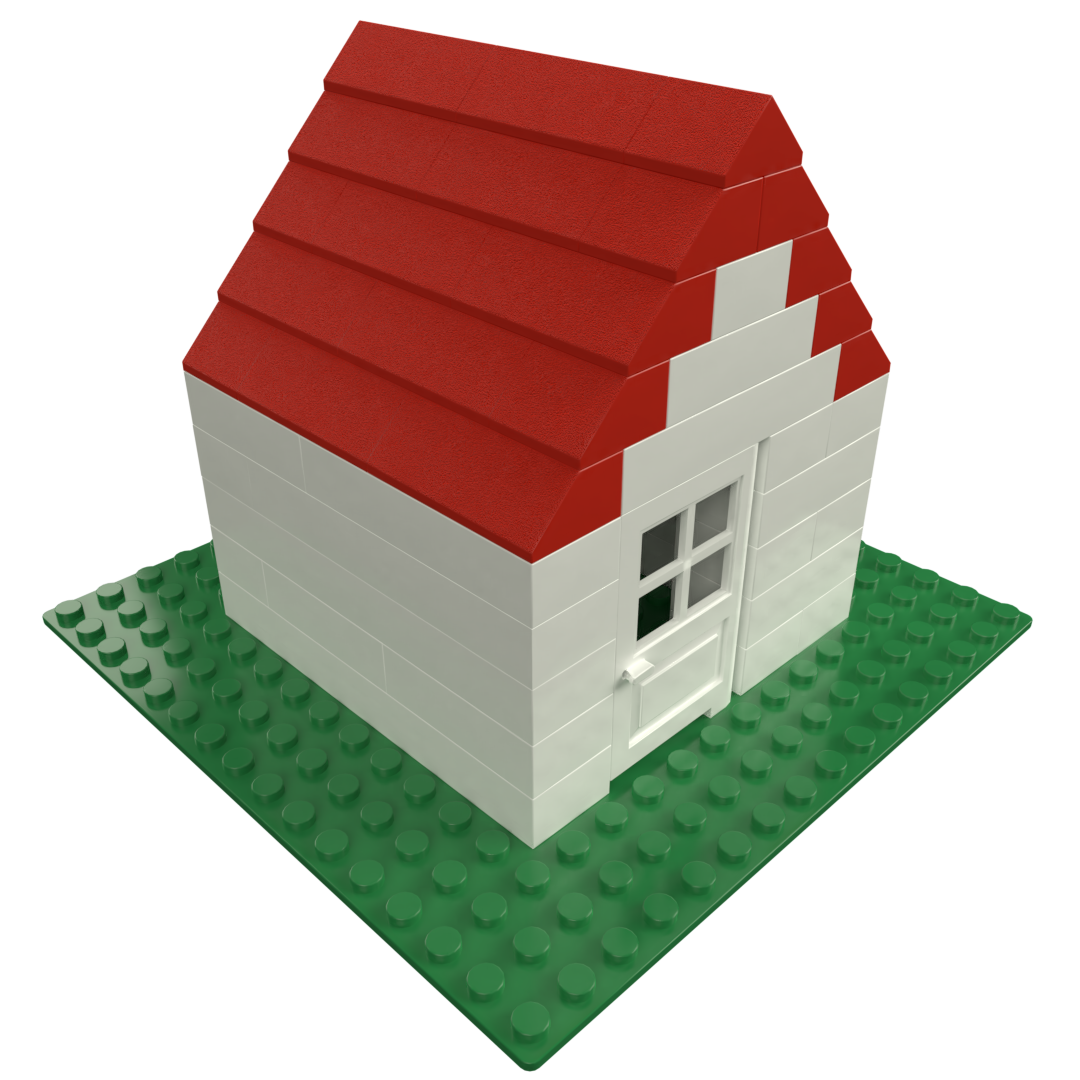
\includegraphics[width=\textwidth]{images/02_modelling_languages/lego_house.png}
    \end{column}\begin{column}{0.45\textwidth}
        \centering
        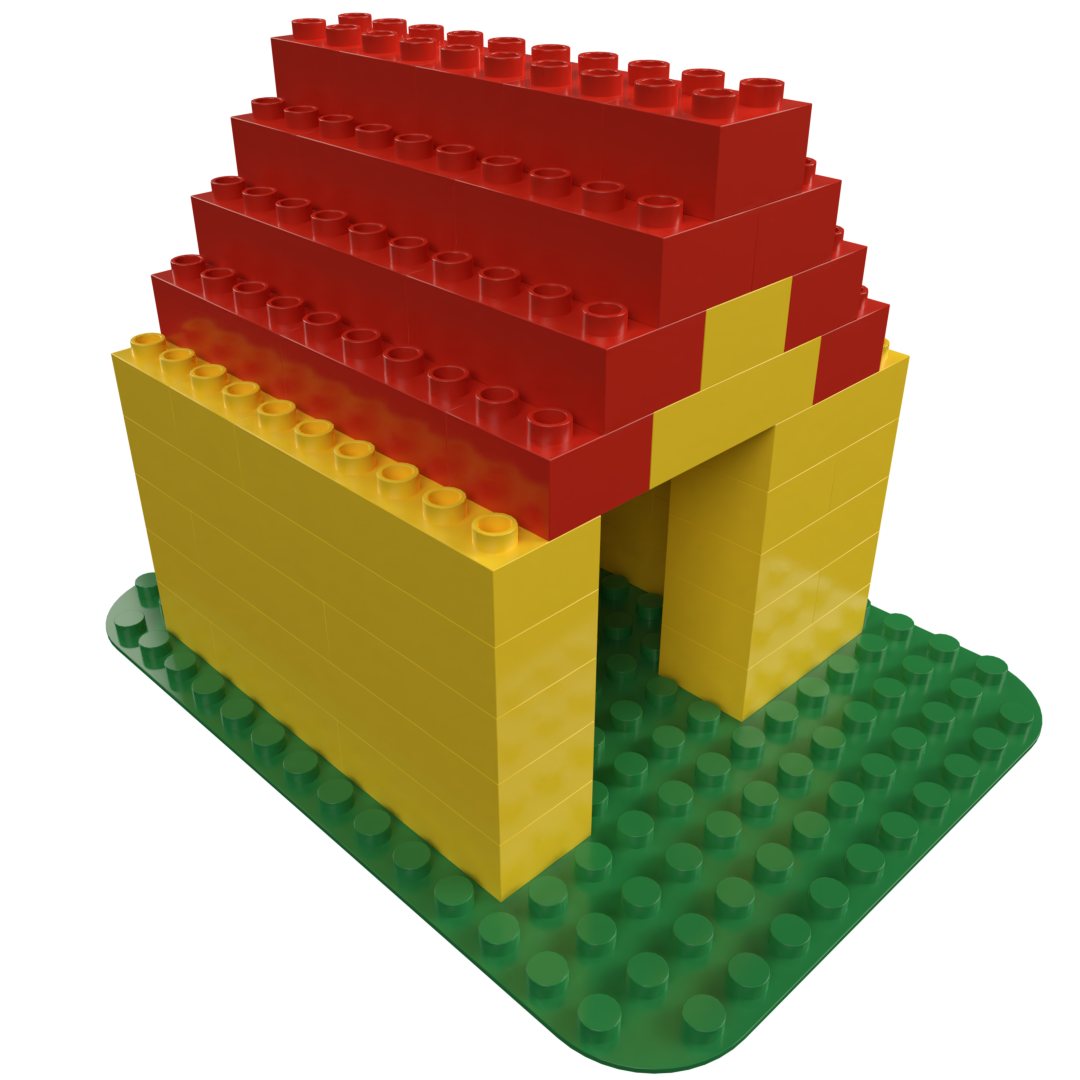
\includegraphics[width=\textwidth]{images/03_transformation_framework/duplo_house.png}
    \end{column}
\end{columns}
\end{frame}

\begin{frame}{Combining transformations}
    \begin{columns}[c]
        \begin{column}{0.05\textwidth}
        \end{column}\begin{column}{0.3\textwidth}
            \centering
            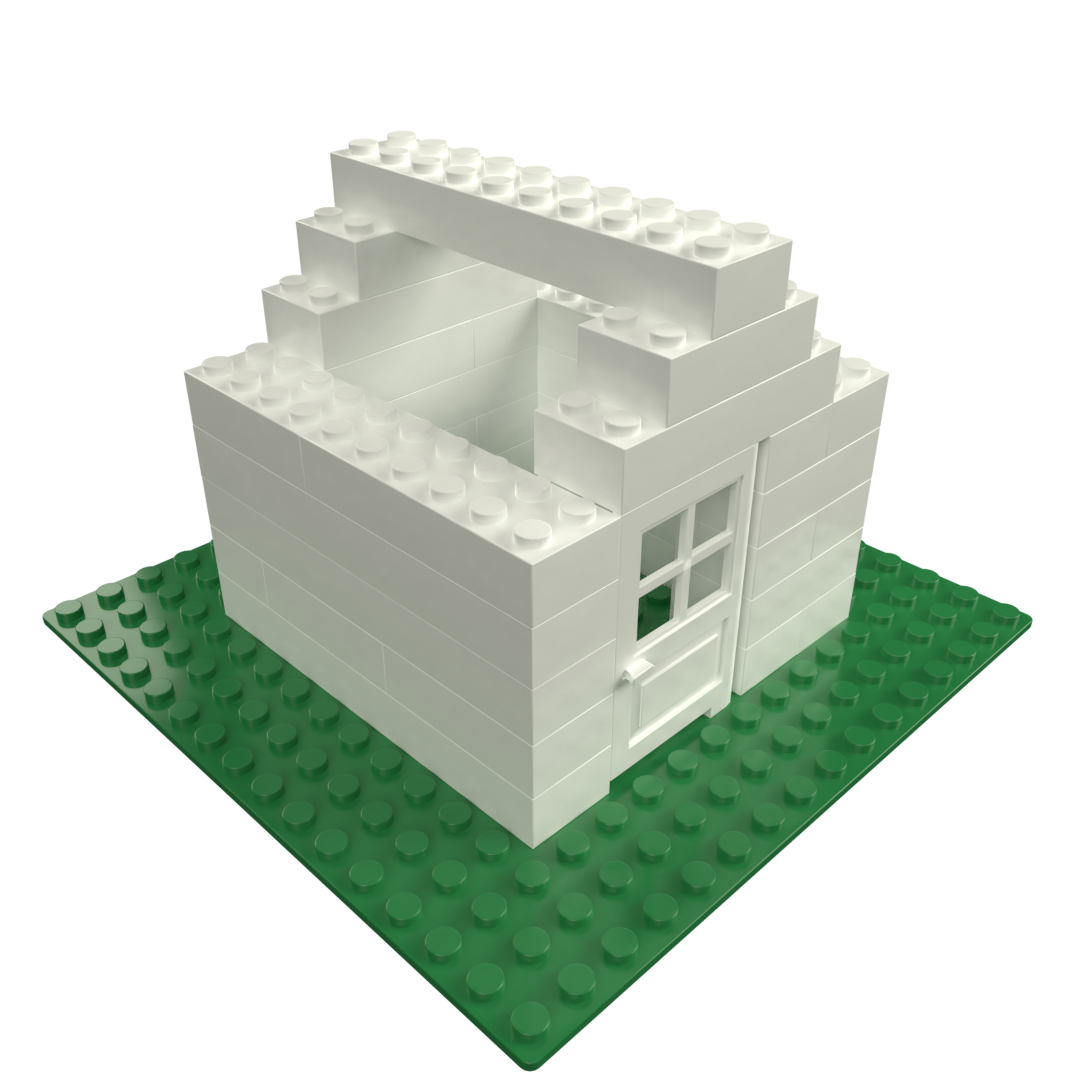
\includegraphics[width=0.7\textwidth]{images/03_transformation_framework/lego_house_roofless.png}
        \end{column}\begin{column}{0.05\textwidth}
            \centering
            +
        \end{column}\begin{column}{0.2\textwidth}
            \centering
            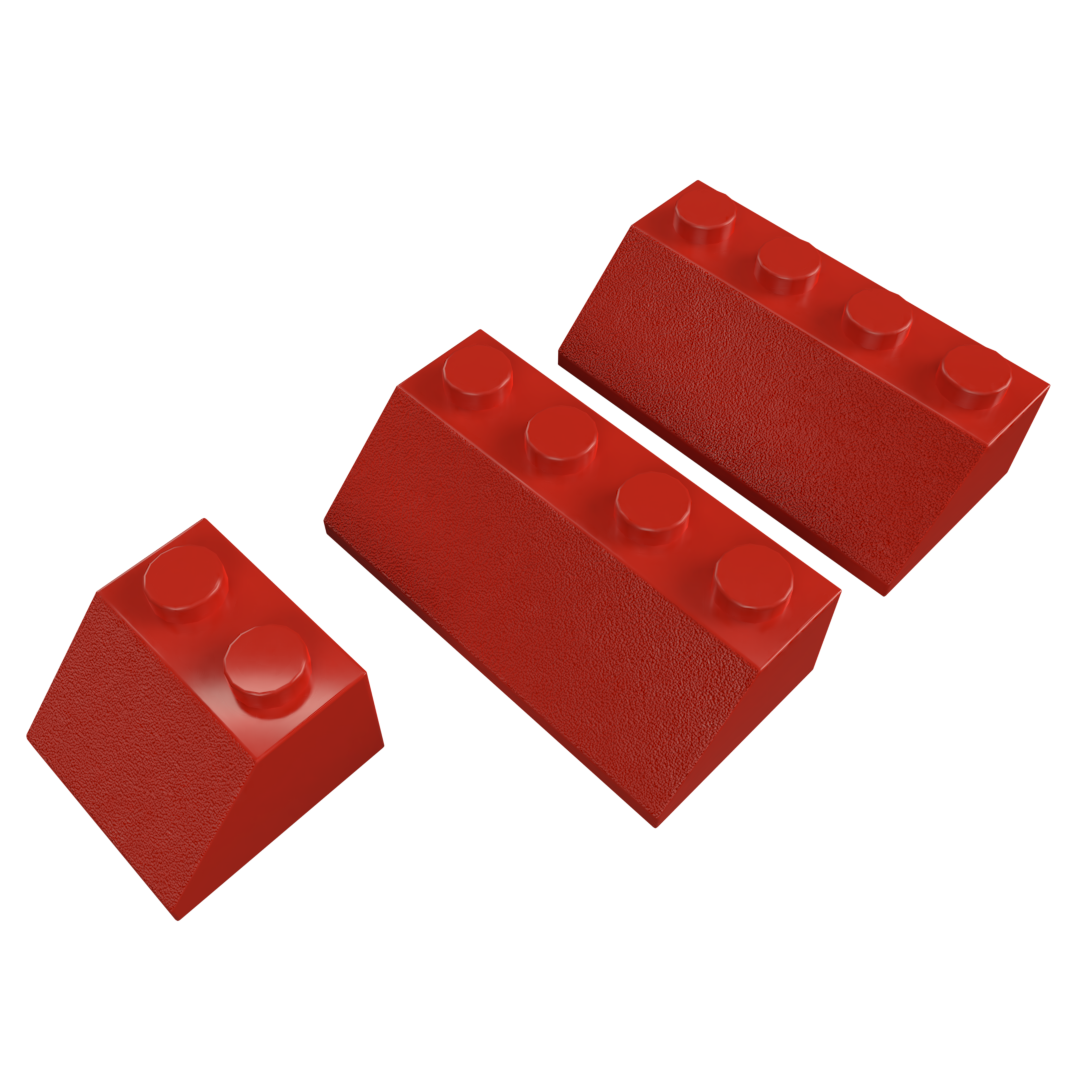
\includegraphics[width=0.7\textwidth]{images/03_transformation_framework/lego_roof_pieces.png}
        \end{column}\begin{column}{0.05\textwidth}
            \centering
            =
        \end{column}\begin{column}{0.3\textwidth}
            \centering
            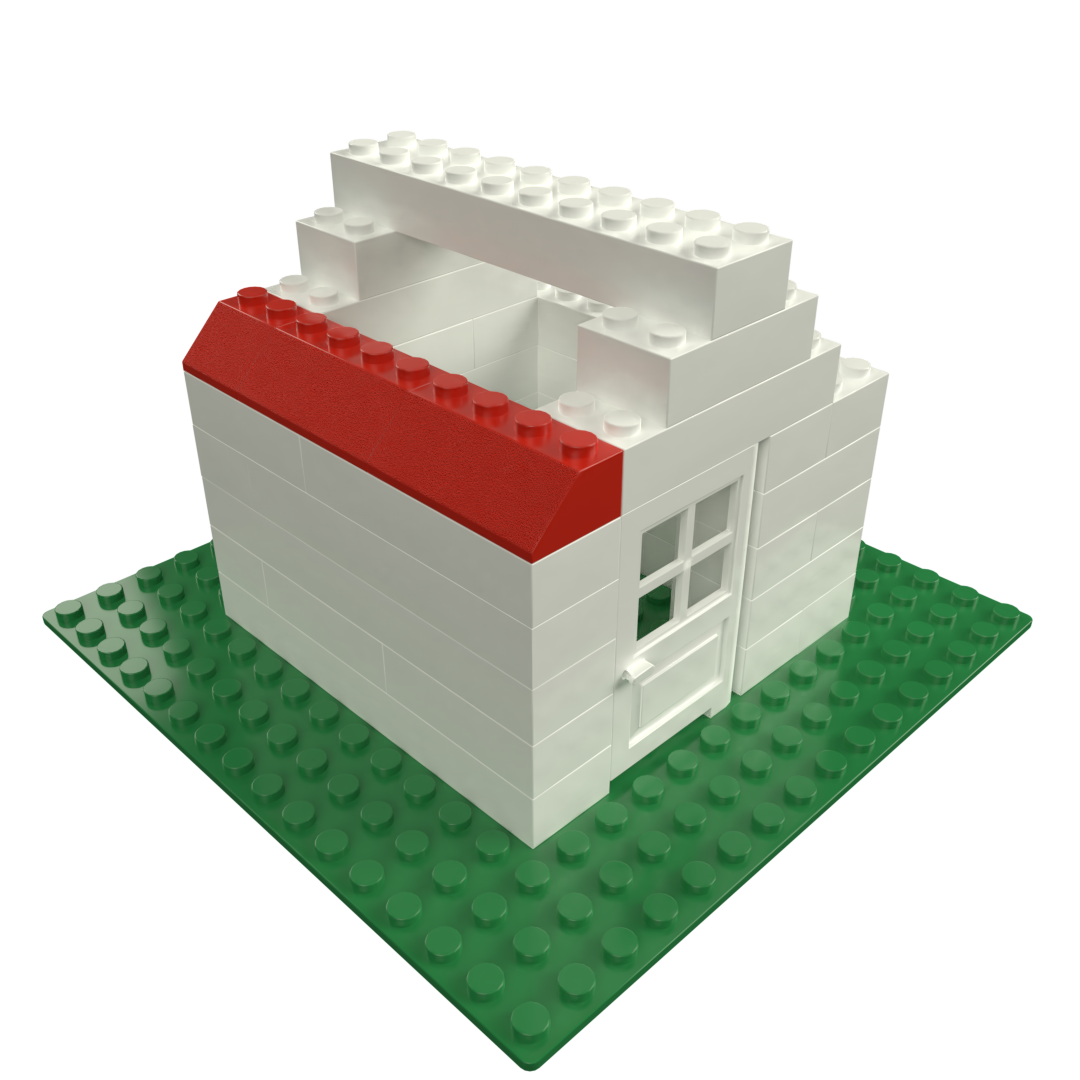
\includegraphics[width=0.7\textwidth]{images/03_transformation_framework/lego_house_roof_step.png}
        \end{column}
    \end{columns}
    \begin{columns}[c]
        \begin{column}{0.05\textwidth}
        \end{column}\begin{column}{0.3\textwidth}
            \centering
            \rotatebox{90}{$\leftrightarrow$}
        \end{column}\begin{column}{0.05\textwidth}
            \centering
            $\sqcup$
        \end{column}\begin{column}{0.2\textwidth}
            \centering
            \rotatebox{90}{$\leftrightarrow$}
        \end{column}\begin{column}{0.05\textwidth}
            \centering
            =
        \end{column}\begin{column}{0.3\textwidth}
            \centering
            \rotatebox{90}{$\leftrightarrow$}
        \end{column}
    \end{columns} 
    \begin{columns}[c]
        \begin{column}{0.05\textwidth}
        \end{column}\begin{column}{0.3\textwidth}
            \centering
            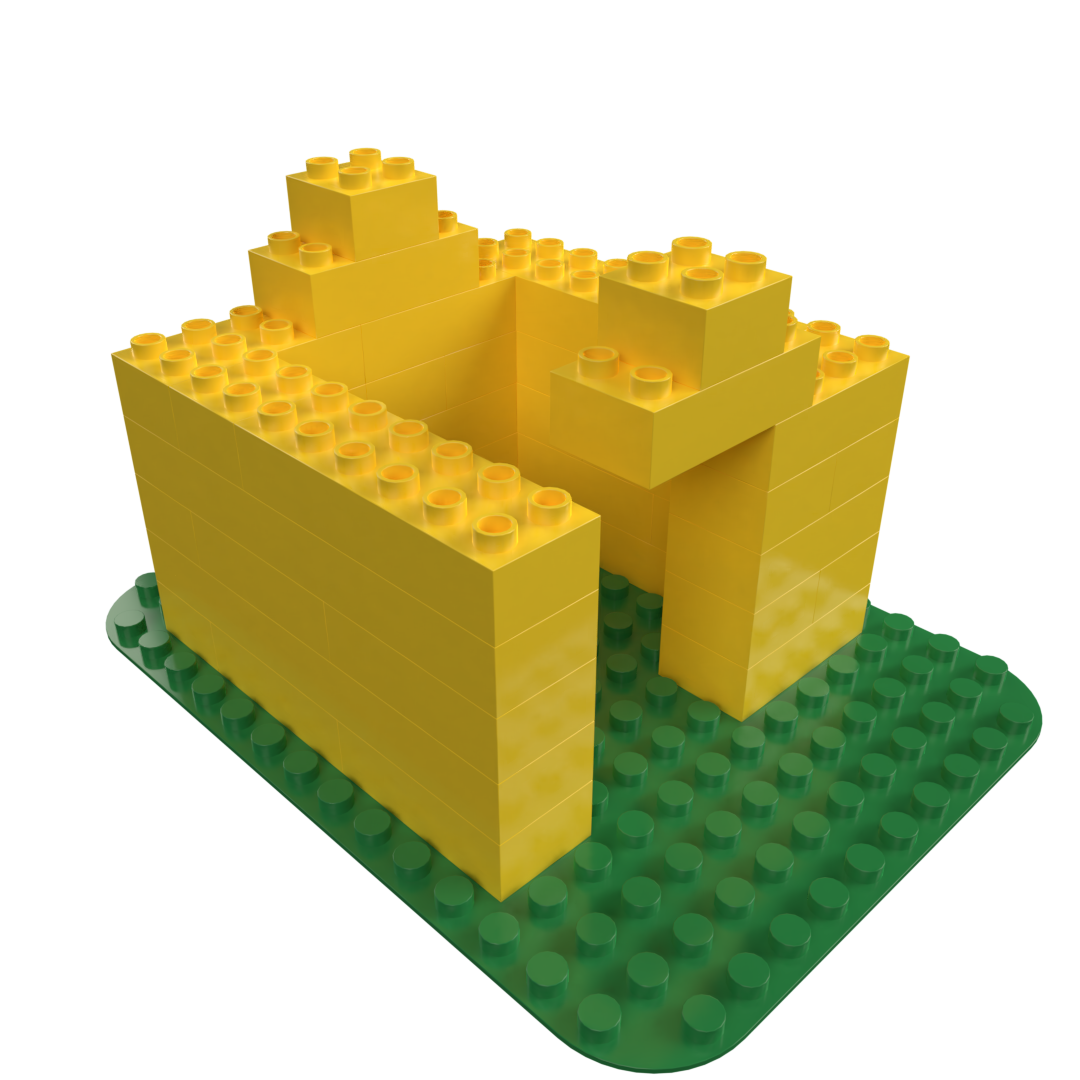
\includegraphics[width=0.7\textwidth]{images/03_transformation_framework/duplo_house_roofless.png}
        \end{column}\begin{column}{0.05\textwidth}
            \centering
            +
        \end{column}\begin{column}{0.2\textwidth}
            \centering
            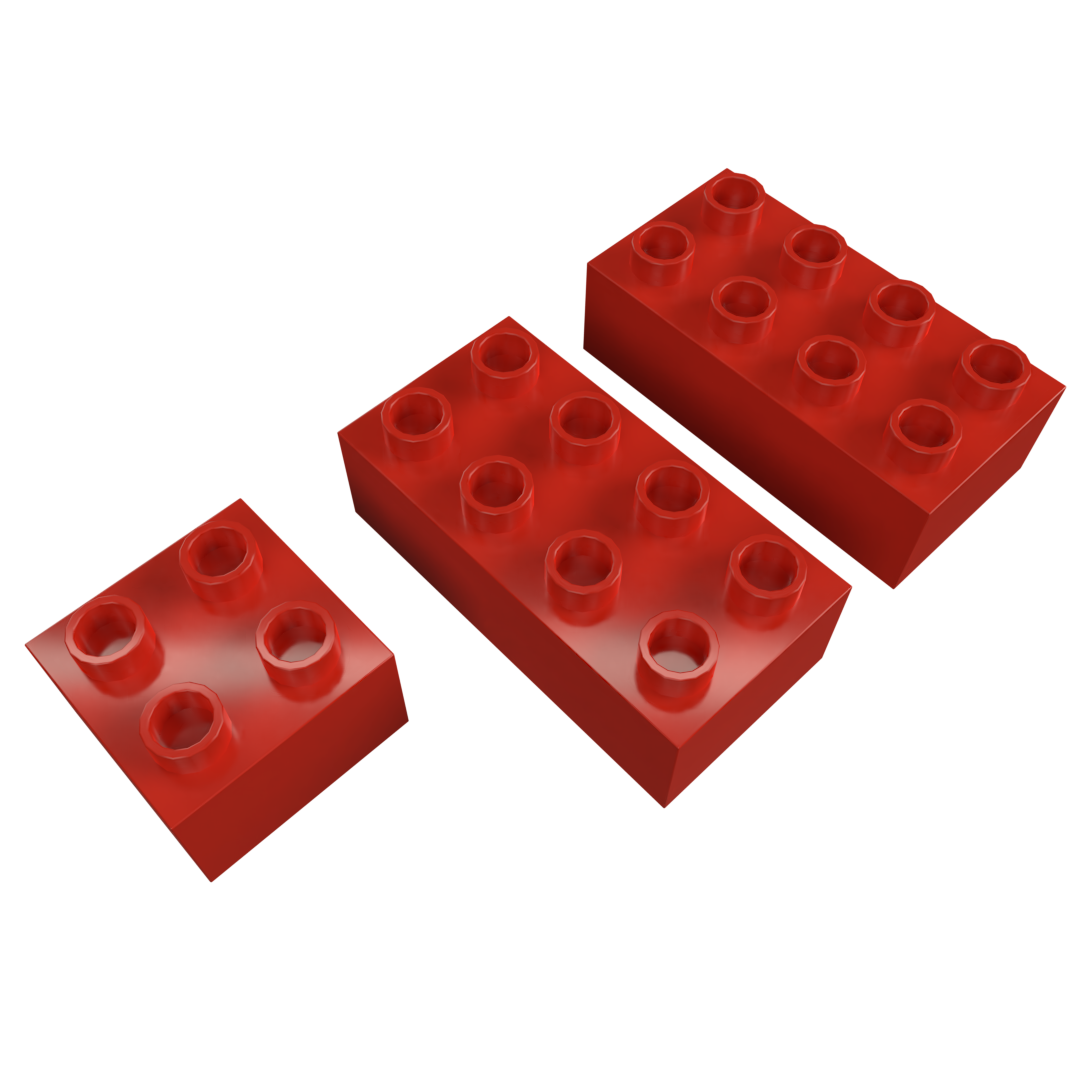
\includegraphics[width=0.7\textwidth]{images/03_transformation_framework/duplo_roof_pieces.png}
        \end{column}\begin{column}{0.05\textwidth}
            \centering
            =
        \end{column}\begin{column}{0.3\textwidth}
            \centering
            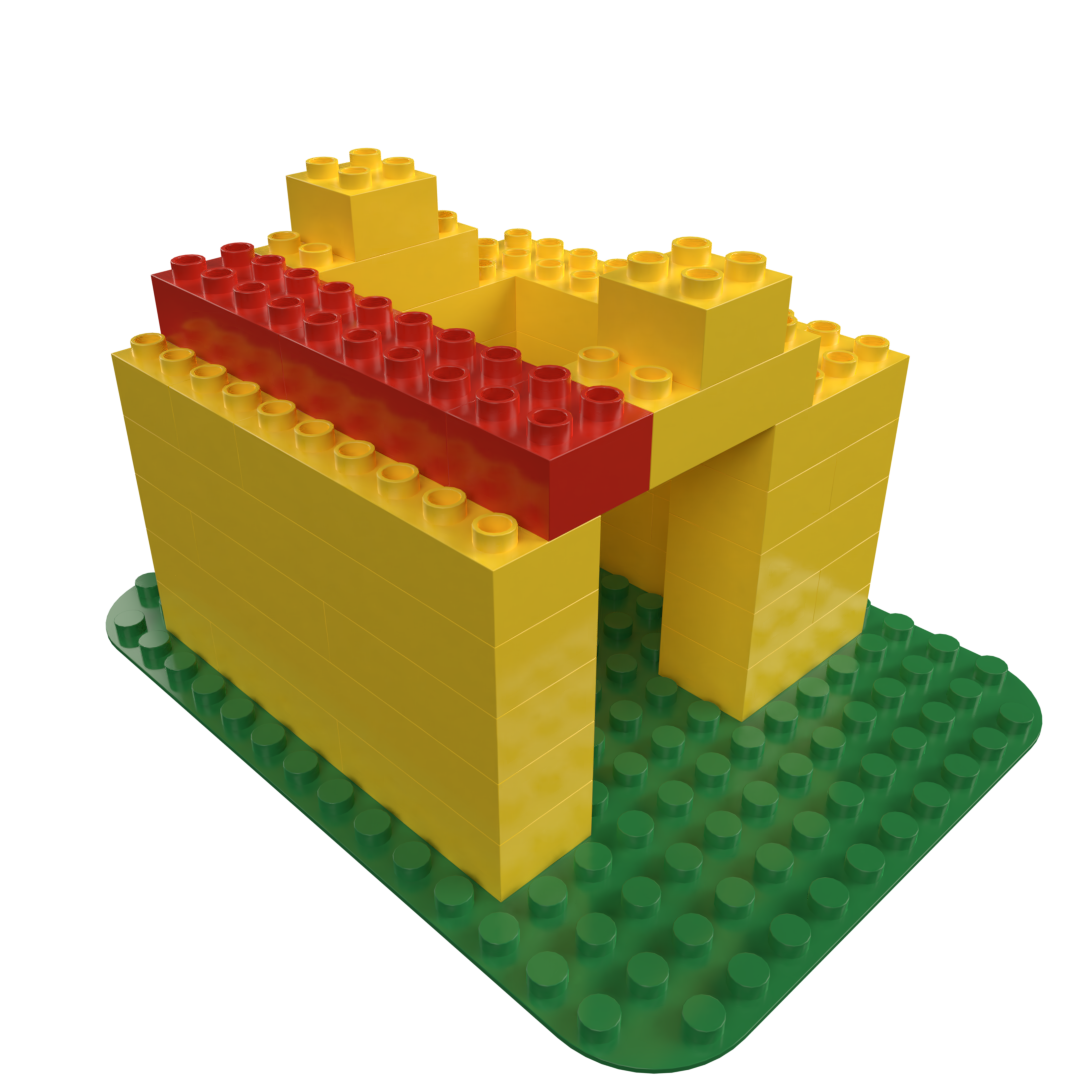
\includegraphics[width=0.7\textwidth]{images/03_transformation_framework/duplo_house_roof_step.png}
        \end{column}
    \end{columns} 
\end{frame}

\begin{frame}{What do we need?}
    \centering
    \begin{tikzpicture} 
    \path
    (-3,4) node[circle,draw,minimum size=10mm,inner sep=0pt](ME) {$E$}
    (-4.5,2) node[circle,draw,minimum size=10mm,inner sep=0pt](MA) {$M_A$}
    (-1.5,2) node[circle,draw,minimum size=10mm,inner sep=0pt](MB) {$M_B$}
    (-3,0) node[circle,draw,minimum size=10mm,inner sep=0pt](MAB) {$M_{AB}$}
    
    (3,4) node[circle,draw,minimum size=10mm,inner sep=0pt](GN) {$N$}
    (1.5,2) node[circle,draw,minimum size=10mm,inner sep=0pt](GA) {$G_A$}
    (4.5,2) node[circle,draw,minimum size=10mm,inner sep=0pt](GB) {$G_B$}
    (3,0) node[circle,draw,minimum size=10mm,inner sep=0pt](GAB) {$G_{AB}$};
    
    \path[]		
    (ME) [-, black, out=240, in=90] edge node[above] {} (MA)
    (ME) [-, black, out=300, in=90] edge node[above] {} (MB)
    
    (MA) [-{Latex[width=5]}, black, out=270, in=90] edge[onslide=<2->{red}] node[above] {} (MAB)
    (MB) [-{Latex[width=5]}, black, out=270, in=90] edge[onslide=<2->{red}] node[above] {} (MAB)
    
    (GN) [-, black, out=240, in=90] edge node[above] {} (GA)
    (GN) [-, black, out=300, in=90] edge node[above] {} (GB)
    
    (GA) [-{Latex[width=5]}, black, out=270, in=90] edge[onslide=<3->{red}] node[above] {} (GAB)
    (GB) [-{Latex[width=5]}, black, out=270, in=90] edge[onslide=<3->{red}] node[above] {} (GAB)
    
    (ME) [-{Latex[width=5]}, black, out=25, in=155] edge node[above] {$f$} (GN)
    (GN) [-{Latex[width=5]}, black, out=165, in=15] edge node[above] {} (ME)
    
    (MA) [-{Latex[width=5]}, black, out=35, in=145] edge node[above] {$f_A$} (GA)
    (GA) [-{Latex[width=5]}, black, out=155, in=25] edge node[above] {} (MA)
    
    (MB) [-{Latex[width=5]}, black, out=35, in=145] edge node[above] {$f_B$} (GB)
    (GB) [-{Latex[width=5]}, black, out=155, in=25] edge node[above] {} (MB)
    
    (MAB) [-{Latex[width=5]}, black, out=25, in=155] edge[onslide=<4->{red}] node[above] {$f_{A} \sqcup f_{B}$} (GAB)
    (GAB) [-{Latex[width=5]}, black, out=165, in=15] edge[onslide=<4->{red}] node[above] {} (MAB)
    ;
    \end{tikzpicture}
\end{frame}

\begin{frame}{What do we need?}
    Type level:
    \begin{itemize}
        \item The combination of type models
        \item The combination of type graphs
        \item The combination of transformation functions between type models and type graphs
    \end{itemize}
    \vspace{0.25cm}
    Instance level:
    \begin{itemize}
        \item The combination of instance models
        \item \alert<2>{The combination of instance graphs}
        \item The combination of transformation functions between instance models and instance graphs
    \end{itemize}
\end{frame}

\note{
	\begin{itemize}
	    \item Explain that to make the transformation framework work, some things need to be defined and proven.
	    \item Explain that the combination of models and graphs is needed.
	    \item Explain that the combination of transformation functions is needed.
	    \item Explain that both are done twice, one time for the type level and one time for the instance level.
	\end{itemize}
}

\begin{frame}{Revisiting instance graphs}
Suppose an instance graph IG typed by type graph TG:
\begin{equation*}
    IG = \langle N, E, ident \rangle
\end{equation*}\pause
\vspace{0.5cm}
Structural properties:
\begin{itemize}
    \item The set of nodes is a subset of the set of valid GROOVE nodes.
    \item The set of edges is a set of triples, with a source node, edge type and target nodes: $E \subseteq N \times ET_{TG} \times N$
    \item The $\mathrm{ident}$ function maps a set of identities to a node in the graph.
\end{itemize}
\end{frame}

\begin{frame}{Revisiting instance graphs}
Suppose an instance graph IG typed by type graph TG:
\begin{equation*}
    IG = \langle N, E, ident \rangle
\end{equation*}
\vspace{0.5cm}
Validity properties:
\begin{itemize}
    \item The nodes $N$ must be properly typed.
    \item The source of each edge $e \in E_{IG}$ must be properly typed.
    \item The target of each edge $e \in E_{IG}$ must be properly typed.
    \item Abstract types cannot have instances.
    \item The outgoing multiplicity of each edge type must be adhered to.
    \item The incoming multiplicity of each edge type must be adhered to.
    \item Nodes must be contained by at most one other node.
    \item There may be no cycle between the containment edges in $E_{IG}$.
\end{itemize}
\end{frame}

\begin{frame}{Revisiting instance graphs}
\begin{columns}[c]
    \begin{column}{0.05\textwidth}
    \end{column}\begin{column}{0.3\textwidth}
        \centering
        % To use this figure in your LaTeX document
% import the package groove/resources/groove2tikz.sty
%
\begin{tikzpicture}[scale=\tikzscale,name prefix=test-]
\node[type_node] (n0) at (2.000, -1.265) {\ml{\textbf{\hspace{0.2cm}A\hspace{0.2cm}}}};
\node[type_node] (n1) at (2.000, -2.3) {\ml{\textbf{\hspace{0.2cm}B\hspace{0.2cm}}}};

\path[basic_edge, composite](n0.south -| 1.800, -2.3) -- node[lab] {\ml{y}} (n1) ;
\path[basic_edge, composite](n1) -- node[lab] {\ml{x}} (n0.south -| 2.200, -1.265) ;
\end{tikzpicture}

    \end{column}\begin{column}{0.3\textwidth}
        \centering
        % To use this figure in your LaTeX document
% import the package groove/resources/groove2tikz.sty
%
\begin{tikzpicture}[scale=\tikzscale,name prefix=start-]
\node[basic_node] (n0) at (0.270, -0.360) {\ml{\textbf{A}}};
\node[basic_node] (n1) at (1.210, -0.760) {\ml{\textbf{B}}};
\node[basic_node] (n2) at (0.280, -1.200) {\ml{\textbf{A}}};

\path[basic_edge] (n0)  -- node[lab] {\ml{y}} (n1) ;
\path[basic_edge] (n1)  -- node[lab] {\ml{x}} (n2) ;
\end{tikzpicture}

    \end{column}\begin{column}{0.3\textwidth}
        \centering
        % To use this figure in your LaTeX document
% import the package groove/resources/groove2tikz.sty
%
\begin{tikzpicture}[scale=\tikzscale,name prefix=invalid-]
\node[basic_node] (n0) at (0.520, -0.450) {\ml{\textbf{A}}};
\node[basic_node] (n1) at (1.350, -0.460) {\ml{\textbf{B}}};

\path[basic_edge](n0.east |- 1.350, -0.530) -- node[below] {\ml{y}} (n1) ;
\path[basic_edge](n1) -- node[above] {\ml{x}} (n0.east |- 0.520, -0.370) ;
\end{tikzpicture}

    \end{column}
\end{columns}
\end{frame}

\note{
	\begin{itemize}
	    \item Revisit instance graphs by explaining the corresponding triple in more detail. Explain that there are structural and validity properties.
	    \item Show an example of the last validity property to have some visualisation of what these properties mean.
	\end{itemize}
}

\begin{frame}{Combination of instance graphs}
\begin{align*}
\mathrm{combine}(IG_A, IG_B) = \langle&
N = N_{IG_A} \cup N_{IG_B} \\&
E = E_{IG_A} \cup E_{IG_B} \\&
\mathrm{ident}(i) =
    \begin{cases}
        \mathrm{ident}_{IG_A}(i) & \mathrm{if }\ i \in \mathrm{dom}\ \mathrm{ident}_{IG_A} \\
        \mathrm{ident}_{IG_B}(i) & \mathrm{if }\ i \in \mathrm{dom}\ \mathrm{ident}_{IG_B} 
    \end{cases}\\ \rangle
\end{align*}
\end{frame}

\note{
	\begin{itemize}
	    \item Explain the definition of instance graphs in more detail. Focus especially on the nodes and edges. Try to argue that it makes sense to just combine the nodes and edges.
	\end{itemize}
}

\begin{frame}{Combination of instance graphs}
    \begin{columns}[c]
        \begin{column}{0.05\textwidth}
        \end{column}\begin{column}{0.25\textwidth}
            \centering
            % To use this figure in your LaTeX document
% import the package groove/resources/groove2tikz.sty
%
\begin{tikzpicture}[scale=1.2, every node/.style={scale=0.6}, name prefix=contact1-]
\node[basic_node] (n0) at (2.685, -3.300) {\ml{\uline{\textit{Example}} : \textbf{Contact}\\email = "networks@example.com"\\firstName = "Networkprofessor"}};

\end{tikzpicture}

        \end{column}\begin{column}{0.05\textwidth}
            \centering
            +
        \end{column}\begin{column}{0.25\textwidth}
            \centering
            % To use this figure in your LaTeX document
% import the package groove/resources/groove2tikz.sty
%
\begin{tikzpicture}[scale=\tikzscale,name prefix=contact2-]
\node[basic_node] (n0) at (1.345, -1.595) {\ml{\uline{\textit{Example}} : \textbf{Contact}\\\textit{fav}}};
\node[basic_node] (n2) at (1.295, -2.985) {\ml{\textbf{Address}\\addressLine = "November Str. 15"\\country = "NL"}};

\path[basic_edge](n0.south -| 1.295, -2.985) -- node[lab] {\ml{addresses}} (n2) ;
\end{tikzpicture}

        \end{column}\begin{column}{0.05\textwidth}
            \centering
            =
        \end{column}\begin{column}{0.3\textwidth}
            \centering
            % To use this figure in your LaTeX document
% import the package groove/resources/groove2tikz.sty
%
\begin{tikzpicture}[scale=1.2, every node/.style={scale=0.6}, name prefix=contact-]
\node[basic_node] (n0) at (1.350, -1.600) {\ml{\textbf{Contact}\\\textit{fav}\\email = "networks@example.com"\\firstName = "Networkprofessor"}};
\node[basic_node] (n2) at (1.300, -2.990) {\ml{\textbf{Address}\\addressLine = "University Str. 15"\\country = "NL"}};

\path[basic_edge](n0.south -| 1.300, -2.990) -- node[lab] {\ml{addresses}} (n2) ;
\end{tikzpicture}

        \end{column}
    \end{columns}
\end{frame}

\begin{frame}{Combination of instance graphs}
Assume that:
\begin{itemize}
    \item $IG_A$ is a valid instance graph typed by $TG_A$.
    \item $IG_B$ is a valid instance graph typed by $TG_B$.
    \item $\mathrm{combine}(TG_A, TG_B)$ is a valid type graph.
    \item All shared identities map to the same node.
\end{itemize}

Then prove using these assumptions that $\mathrm{combine}(IG_A, IG_B)$ (typed by $\mathrm{combine}(TG_A, TG_B)$) is valid.
\end{frame}

\note{
	\begin{itemize}
	    \item Explain that within the transformation framework, a proof for the combination of instance graphs is given with the assumption that $IG_A$ and $IG_B$ are valid, as well as their combination of type graphs.
	\end{itemize}
}

\begin{frame}{Combination of instance graphs}
\begin{proof}
To prove that $\mathrm{combine}(IG_A, IG_B)$ is valid, show that each of the structural properties for a valid instance graph and all the validity properties for a valid instance graph hold.
\end{proof}
\end{frame}

\note{
	\begin{itemize}
	    \item Explain what the proof looks like. It is basically proving all the properties under assumptions.
	\end{itemize}
}

\begin{frame}{Combination of instance graphs}
The source of each edge $e \in E_{IG}$ must be properly typed:\\
$\forall e \in E_{\mathrm{combine}(IG_A, IG_B)}\!: \mathrm{type}_n \big(\mathrm{src}(e)\big) \sqsubseteq_{\mathrm{combine}(TG_A, TG_B)} \mathrm{src} \big(\mathrm{type}_e(e)\big)$
\pause

\begin{proof}
Make a case distinction. $e \in E_{\mathrm{combine}(IG_A, IG_B)} \implies e \in E_{IG_A} \lor e \in E_{IG_B}$.\\
\vspace{0.2cm}
If $e \in E_{IG_A}$, then $\mathrm{type}_n \big(\mathrm{src}(e)\big) \sqsubseteq_{TG_{A}} \mathrm{src} \big(\mathrm{type}_e(e)\big)$, since $IG_A$ is valid. Types are preserved after combination.
Furthermore, because of the definition of $\mathrm{combine}(TG_A, TG_B)$, have that $\mathrm{type}_n \big(\mathrm{src}(e)\big) \sqsubseteq_{\mathrm{combine}(TG_A, TG_B)} \mathrm{src} \big(\mathrm{type}_e(e)\big)$.\\
\vspace{0.2cm}
The case for $e \in E_{IG_B}$ is similar.
\end{proof}
\end{frame}

\note{
	\begin{itemize}
	    \item Explain one property, the source of each edge must be properly typed. Introduce the first order logic equivalent of this statement.
	    \item Show the proof. Explain that if an edge is in the combination, it was in one of the two graphs. For each case, you can proof that it is also typed correctly in the combination.
	\end{itemize}
}
\section{Library of transformations}

\begin{frame}{The library}
    The library of transformations contains small transformation steps that are proven correct.
    \begin{itemize}
        \item Each transformation in here can be used as building block.
        \item The library of transformations does not achieve complete coverage.
    \end{itemize}
\end{frame}

\note{
	\begin{itemize}
	    \item Explain what the library of transformations is.
	    \item Explain that the library included within this work is incomplete, e.g. not all possible models can be build from this library.
	    \item Explain in context what the library of transformations is.
	\end{itemize}
}

\begin{frame}{In context}
    \begin{columns}[c]
        \begin{column}{0.05\textwidth}
        \end{column}\begin{column}{0.3\textwidth}
            \centering
            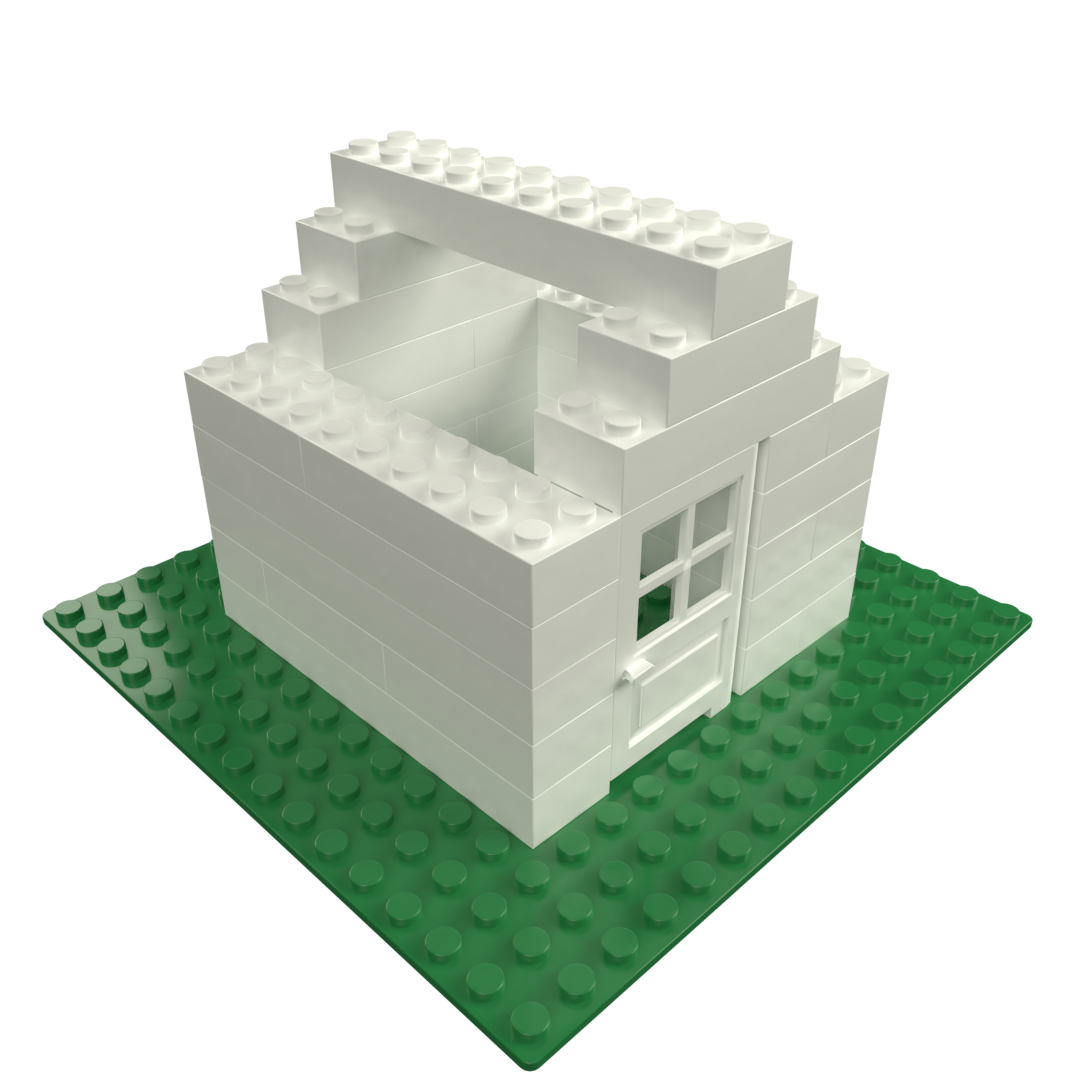
\includegraphics[width=0.7\textwidth]{images/03_transformation_framework/lego_house_roofless.png}
        \end{column}\begin{column}{0.05\textwidth}
            \centering
            +
        \end{column}\begin{column}{0.2\textwidth}
            \centering
            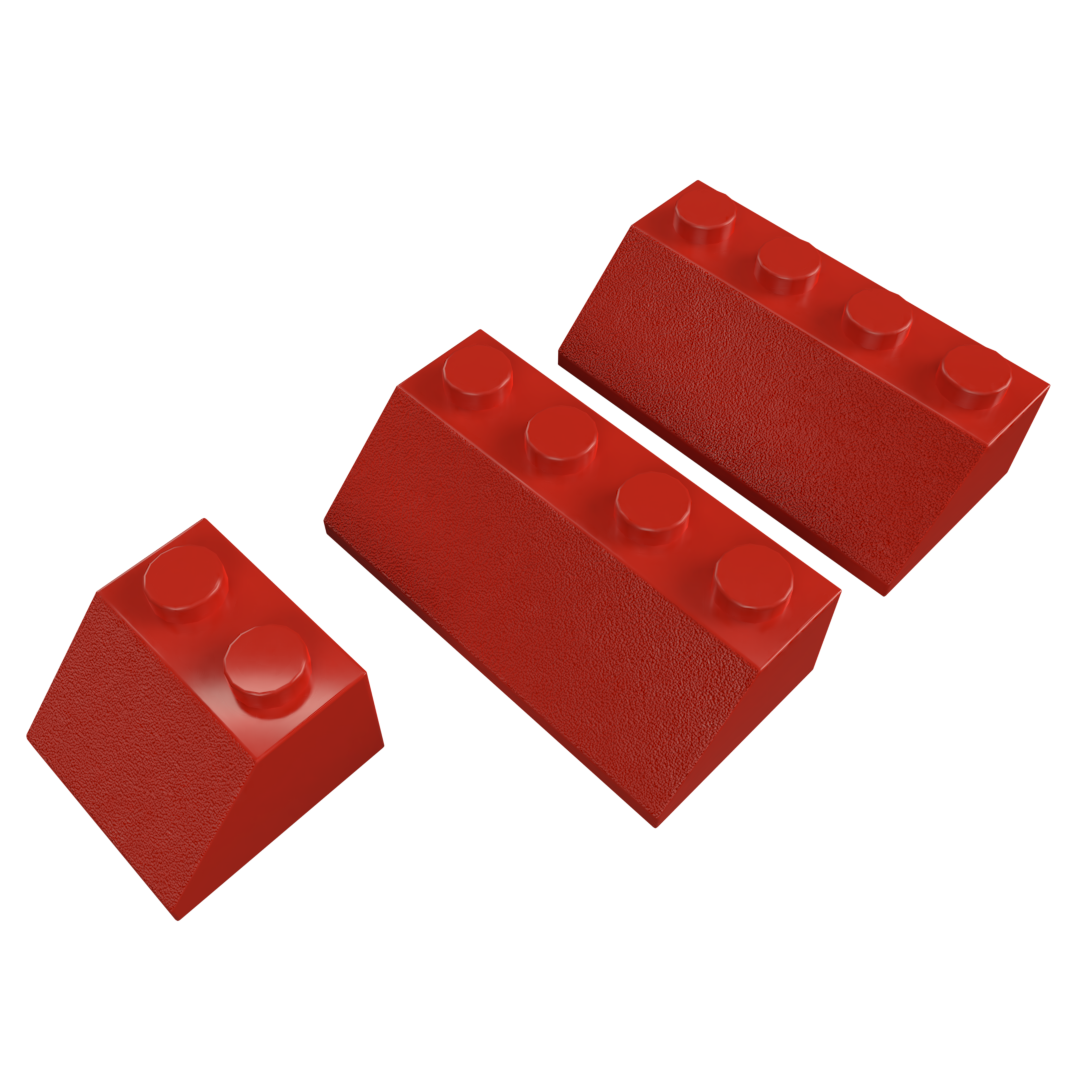
\includegraphics[width=0.7\textwidth]{images/03_transformation_framework/lego_roof_pieces.png}
        \end{column}\begin{column}{0.05\textwidth}
            \centering
            =
        \end{column}\begin{column}{0.3\textwidth}
            \centering
            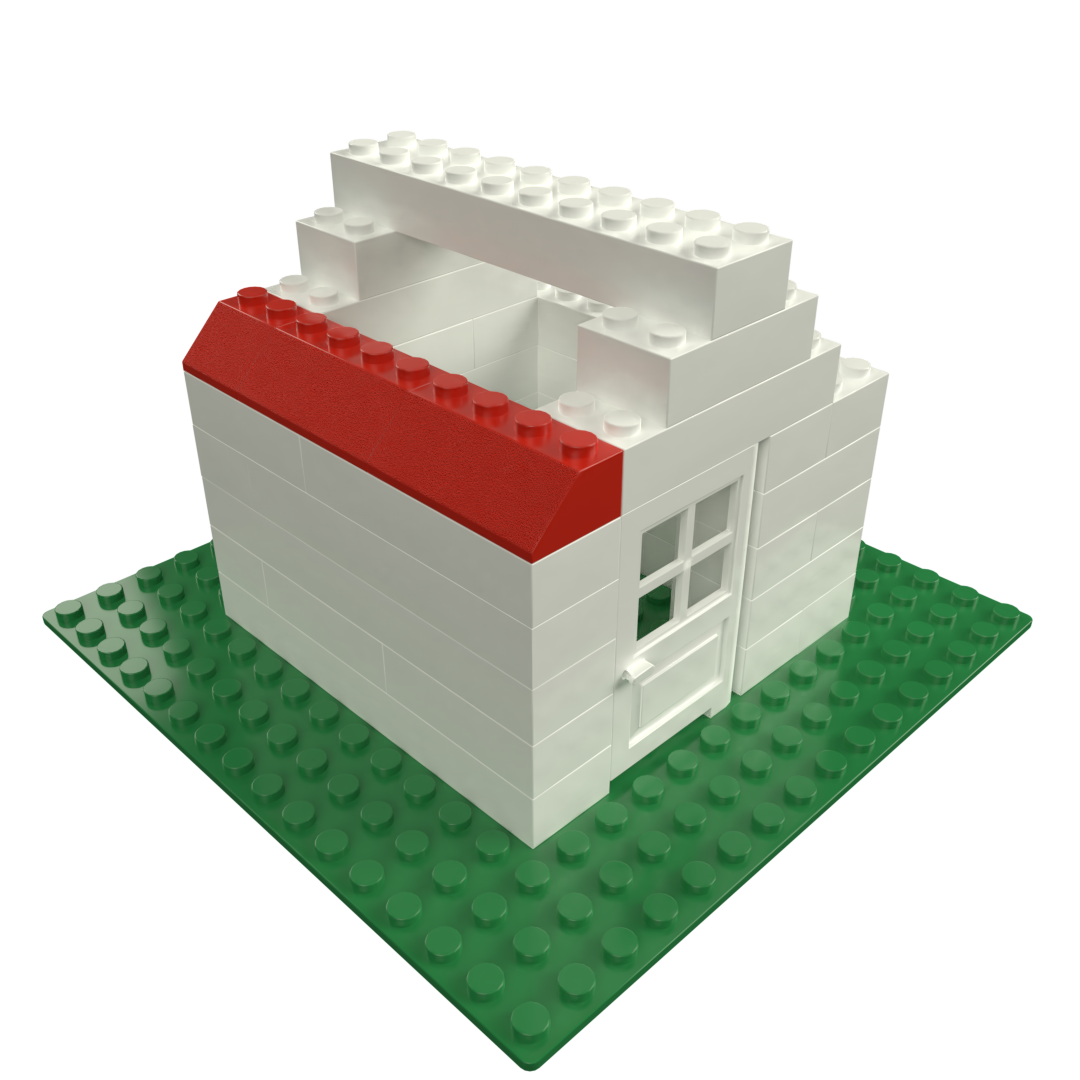
\includegraphics[width=0.7\textwidth]{images/03_transformation_framework/lego_house_roof_step.png}
        \end{column}
    \end{columns}
    \begin{columns}[c]
        \begin{column}{0.05\textwidth}
        \end{column}\begin{column}{0.3\textwidth}
            \centering
            \rotatebox{90}{$\leftrightarrow$}
        \end{column}\begin{column}{0.05\textwidth}
            \centering
            $\sqcup$
        \end{column}\begin{column}{0.2\textwidth}
            \centering
            \rotatebox{90}{$\leftrightarrow$}
        \end{column}\begin{column}{0.05\textwidth}
            \centering
            =
        \end{column}\begin{column}{0.3\textwidth}
            \centering
            \rotatebox{90}{$\leftrightarrow$}
        \end{column}
    \end{columns} 
    \begin{columns}[c]
        \begin{column}{0.05\textwidth}
        \end{column}\begin{column}{0.3\textwidth}
            \centering
            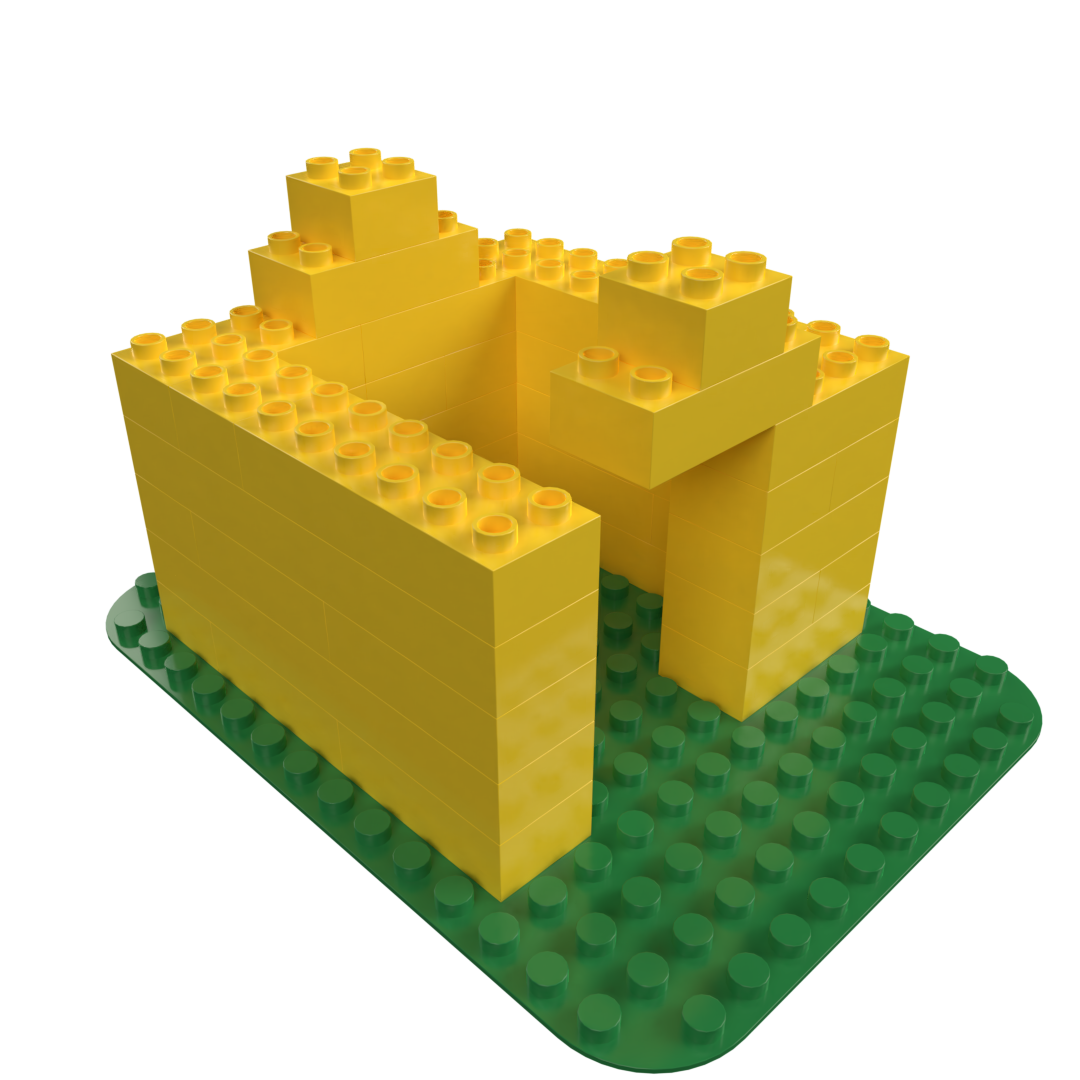
\includegraphics[width=0.7\textwidth]{images/03_transformation_framework/duplo_house_roofless.png}
        \end{column}\begin{column}{0.05\textwidth}
            \centering
            +
        \end{column}\begin{column}{0.2\textwidth}
            \centering
            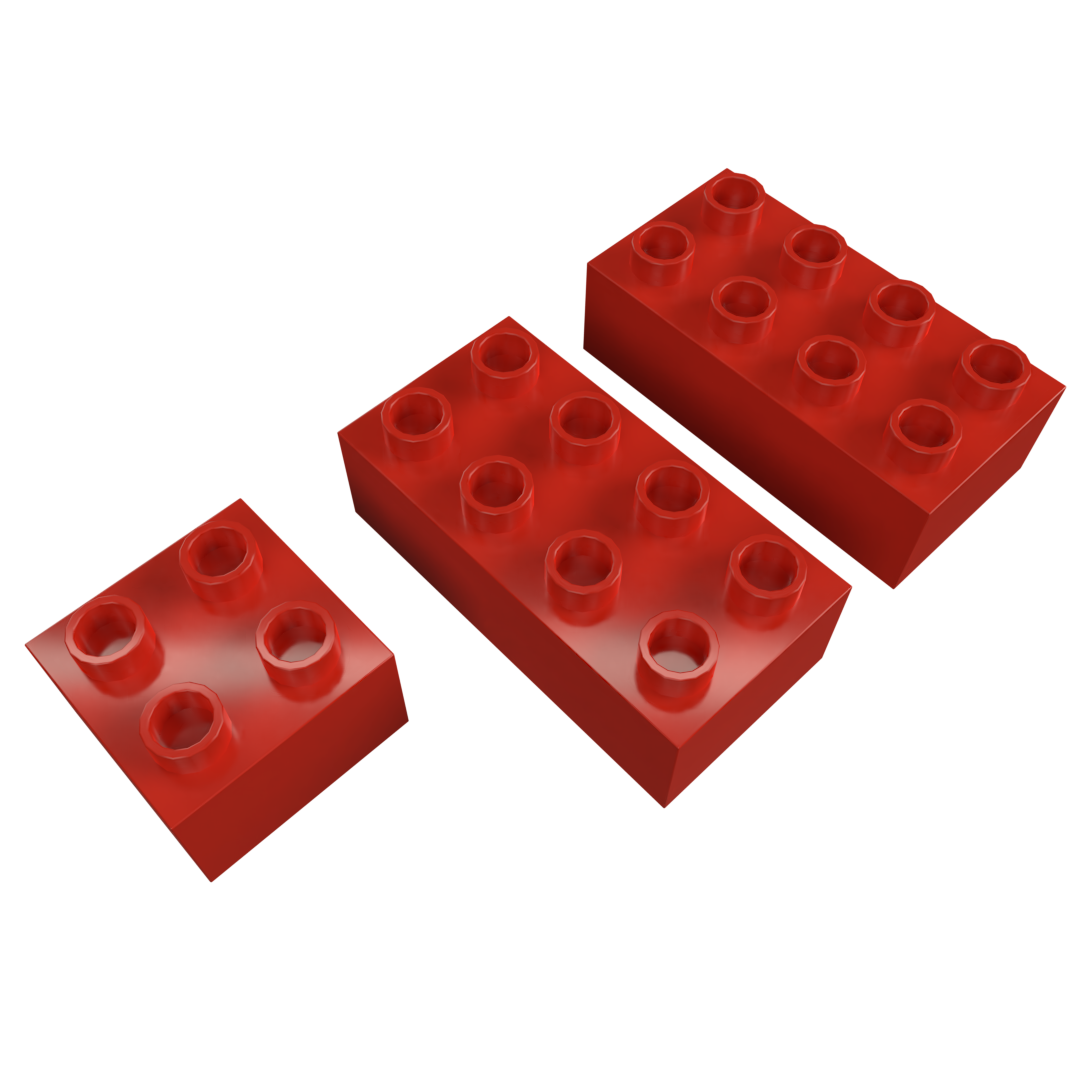
\includegraphics[width=0.7\textwidth]{images/03_transformation_framework/duplo_roof_pieces.png}
        \end{column}\begin{column}{0.05\textwidth}
            \centering
            =
        \end{column}\begin{column}{0.3\textwidth}
            \centering
            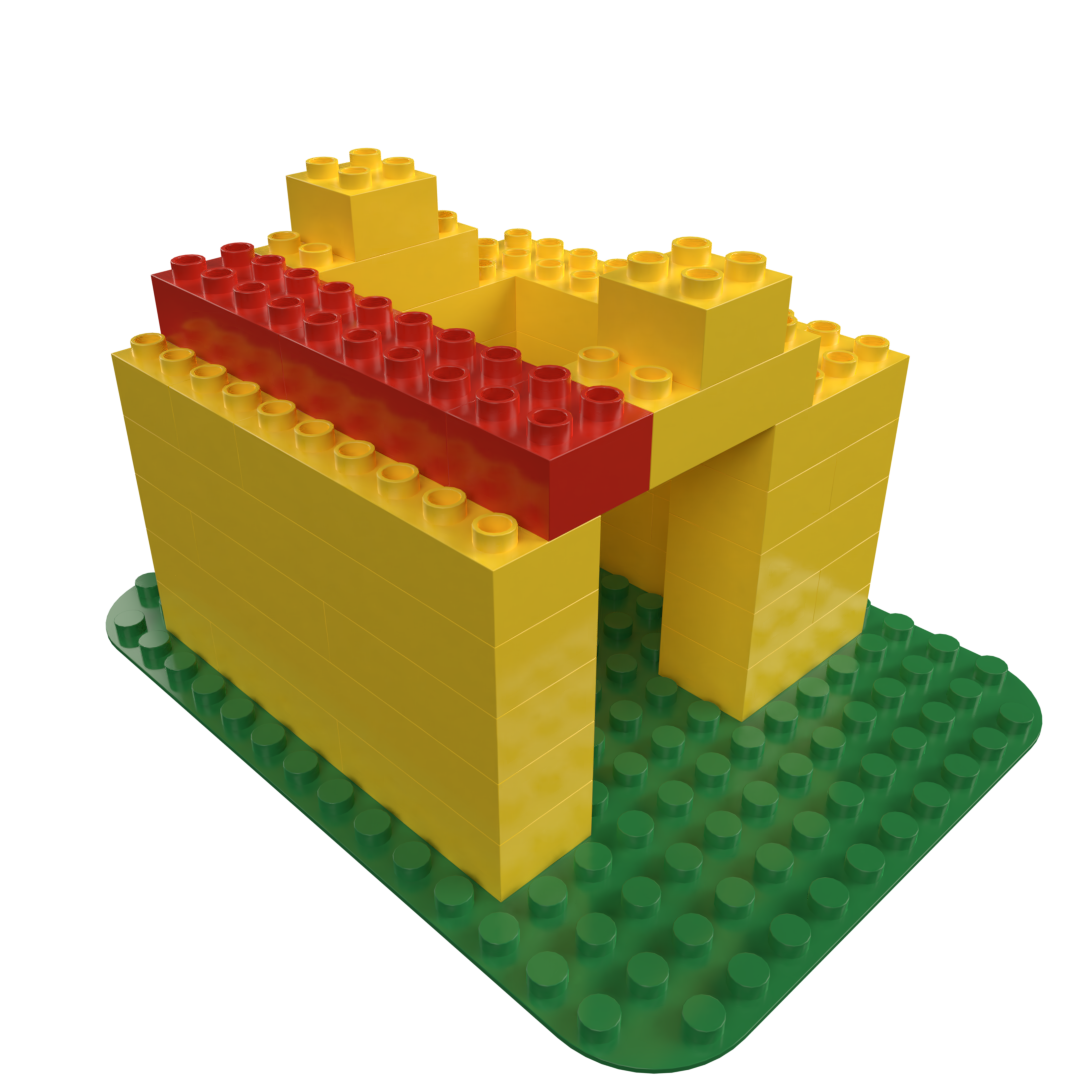
\includegraphics[width=0.7\textwidth]{images/03_transformation_framework/duplo_house_roof_step.png}
        \end{column}
    \end{columns} 
\end{frame}

\begin{frame}{Adding a regular class with instances}
Add a class named \textit{Example} to a model. On the instance level, introduce a set of objects with this type.
\begin{columns}[c]
    \begin{column}{0.05\textwidth}
    \end{column}\begin{column}{0.45\textwidth}
        \centering
        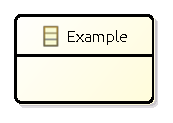
\includegraphics[width=0.5\textwidth]{images/04_library_of_transformations/class_type.pdf}
    \end{column}\begin{column}{0.05\textwidth}
        \centering
        $\leftrightarrow$
    \end{column}\begin{column}{0.45\textwidth}
        \centering
        % To use this figure in your LaTeX document
% import the package groove/resources/groove2tikz.sty
%
\begin{tikzpicture}[scale=\tikzscale,name prefix=test-]
\node[type_node] (n0) at (0.950, -0.850) {\ml{\textbf{Example}}};

\end{tikzpicture}

    \end{column}
\end{columns}
\begin{columns}[c]
    \begin{column}{0.05\textwidth}
    \end{column}\begin{column}{0.45\textwidth}
        \centering
        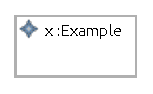
\includegraphics[width=0.5\textwidth]{images/04_library_of_transformations/class_instance.pdf}
    \end{column}\begin{column}{0.05\textwidth}
        \centering
        $\leftrightarrow$
    \end{column}\begin{column}{0.45\textwidth}
        \centering
        % To use this figure in your LaTeX document
% import the package groove/resources/groove2tikz.sty
%
\begin{tikzpicture}[scale=\tikzscale,name prefix=start-]
\node[basic_node] (n0) at (1.620, -0.370) {\ml{\uline{\textit{x}} : \textbf{Example}}};

\end{tikzpicture}

    \end{column}
\end{columns}
\end{frame}

\note{
	\begin{itemize}
	    \item Shortly explain what a transformation within the library looks like. It has a type level transformation with corresponding instance level transformations.
	    \item Very quickly explain the model and how to apply it.
	\end{itemize}
}

\begin{frame}{Adding a string field}
Add a field, typed by a string, named \textit{field} to an existing class named \textit{Example}. For all existing objects typed by \textit{Example}, introduce a new value for the field \textit{field}.
\begin{columns}[c]
    \begin{column}{0.05\textwidth}
    \end{column}\begin{column}{0.45\textwidth}
        \centering
        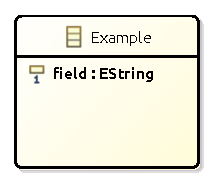
\includegraphics[width=0.7\textwidth]{images/04_library_of_transformations/data_field.pdf}
    \end{column}\begin{column}{0.05\textwidth}
        \centering
        $\leftrightarrow$
    \end{column}\begin{column}{0.45\textwidth}
        \centering
        % To use this figure in your LaTeX document
% import the package groove/resources/groove2tikz.sty
%
\begin{tikzpicture}[scale=\tikzscale,name prefix=test-]
\node[type_node] (n0) at (0.955, -0.775) {\ml{\textbf{Example}\\field: \textbf{string}}};

\end{tikzpicture}

    \end{column}
\end{columns}
\begin{columns}[c]
    \begin{column}{0.05\textwidth}
    \end{column}\begin{column}{0.45\textwidth}
        \centering
        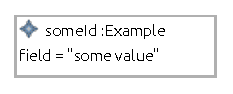
\includegraphics[width=0.7\textwidth]{images/04_library_of_transformations/data_field_value.pdf}
    \end{column}\begin{column}{0.05\textwidth}
        \centering
        $\leftrightarrow$
    \end{column}\begin{column}{0.45\textwidth}
        \centering
        % To use this figure in your LaTeX document
% import the package groove/resources/groove2tikz.sty
%
\begin{tikzpicture}[scale=\tikzscale,name prefix=start-]
\node[basic_node] (n0) at (1.595, -0.775) {\ml{\uline{\textit{someId}} : \textbf{Example}\\field = "some value"}};

\end{tikzpicture}

    \end{column}
\end{columns}
\end{frame}

\note{
	\begin{itemize}
	    \item Explain the addition of a string field as last example.
	\end{itemize}
}
\section{Application}

\begin{frame}{Example application}
    Combine the transformation framework and library of transformations to compose model transformations between Ecore and GROOVE.
    \begin{itemize}
        \item Small contact application, only names and addresses
    \end{itemize}
\end{frame}

\note{
	\begin{itemize}
	    \item Explain that we will see an example of how the transformation framework can be applied.
	    \item The library of transformation is used as the building blocks.
	    \item A small contacts application, only containing names and addresses is discussed.
	\end{itemize}
}

\begin{frame}{Example application}
    \centering
    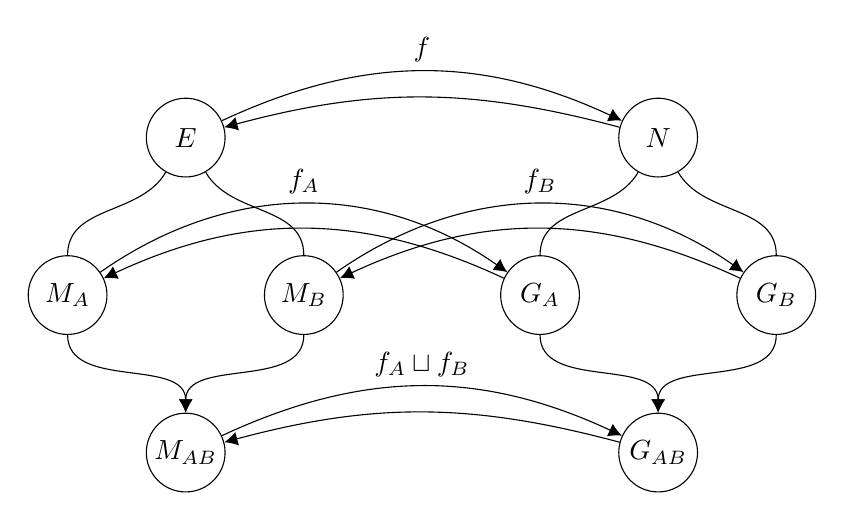
\begin{tikzpicture} 
    \path
    (-3,4) node[circle,draw,minimum size=10mm,inner sep=0pt](ME) {$E$}
    (-4.5,2) node[circle,draw,minimum size=10mm,inner sep=0pt](MA) {$M_A$}
    (-1.5,2) node[circle,draw,minimum size=10mm,inner sep=0pt](MB) {$M_B$}
    (-3,0) node[circle,draw,minimum size=10mm,inner sep=0pt](MAB) {$M_{AB}$}
    
    (3,4) node[circle,draw,minimum size=10mm,inner sep=0pt](GN) {$N$}
    (1.5,2) node[circle,draw,minimum size=10mm,inner sep=0pt](GA) {$G_A$}
    (4.5,2) node[circle,draw,minimum size=10mm,inner sep=0pt](GB) {$G_B$}
    (3,0) node[circle,draw,minimum size=10mm,inner sep=0pt](GAB) {$G_{AB}$};
    
    \path[]		
    (ME) [-, black, out=240, in=90] edge node[above] {} (MA)
    (ME) [-, black, out=300, in=90] edge node[above] {} (MB)
    
    (MA) [-{Latex[width=5]}, black, out=270, in=90] edge node[above] {} (MAB)
    (MB) [-{Latex[width=5]}, black, out=270, in=90] edge node[above] {} (MAB)
    
    (GN) [-, black, out=240, in=90] edge node[above] {} (GA)
    (GN) [-, black, out=300, in=90] edge node[above] {} (GB)
    
    (GA) [-{Latex[width=5]}, black, out=270, in=90] edge node[above] {} (GAB)
    (GB) [-{Latex[width=5]}, black, out=270, in=90] edge node[above] {} (GAB)
    
    (ME) [-{Latex[width=5]}, black, out=25, in=155] edge node[above] {$f$} (GN)
    (GN) [-{Latex[width=5]}, black, out=165, in=15] edge node[above] {} (ME)
    
    (MA) [-{Latex[width=5]}, black, out=35, in=145] edge node[above] {$f_A$} (GA)
    (GA) [-{Latex[width=5]}, black, out=155, in=25] edge node[above] {} (MA)
    
    (MB) [-{Latex[width=5]}, black, out=35, in=145] edge node[above] {$f_B$} (GB)
    (GB) [-{Latex[width=5]}, black, out=155, in=25] edge node[above] {} (MB)
    
    (MAB) [-{Latex[width=5]}, black, out=25, in=155] edge node[above] {$f_{A} \sqcup f_{B}$} (GAB)
    (GAB) [-{Latex[width=5]}, black, out=165, in=15] edge node[above] {} (MAB)
    ;
    \end{tikzpicture}
\end{frame}

\note{
	\begin{itemize}
	    \item Explain how the steps will be repeated.
	\end{itemize}
}

\newcommand\typeframe[3]{
\begin{frame}{Step #3/6: Type level}
    \vspace{-0.55cm}
    \begin{columns}[c]
        \begin{column}{0.06\textwidth}
        \end{column}\begin{column}{0.3\textwidth}
            \centering
            \includegraphics[width=0.66\textwidth]{images/05_application/type_model/step#1.pdf}
        \end{column}\begin{column}{0.015\textwidth}
            \centering
            +
        \end{column}\begin{column}{0.3\textwidth}
            \centering
            \includegraphics[width=0.66\textwidth]{images/05_application/type_model/step#2.pdf}
        \end{column}\begin{column}{0.015\textwidth}
            \centering
            =
        \end{column}\begin{column}{0.3\textwidth}
            \centering
            \includegraphics[width=0.66\textwidth]{images/05_application/type_model/step#3.pdf}
        \end{column}
    \end{columns}
    \begin{columns}[c]
        \begin{column}{0.06\textwidth}
        \end{column}\begin{column}{0.3\textwidth}
            \centering
            \rotatebox{90}{$\leftrightarrow$}
        \end{column}\begin{column}{0.015\textwidth}
            \centering
            $\sqcup$
        \end{column}\begin{column}{0.3\textwidth}
            \centering
            \rotatebox{90}{$\leftrightarrow$}
        \end{column}\begin{column}{0.015\textwidth}
            \centering
            =
        \end{column}\begin{column}{0.3\textwidth}
            \centering
            \rotatebox{90}{$\leftrightarrow$}
        \end{column}
    \end{columns} 
    \begin{columns}[c]
        \begin{column}{0.06\textwidth}
        \end{column}\begin{column}{0.3\textwidth}
            \centering
            \input{images/05_application/type_graph/step#1.tikz}
        \end{column}\begin{column}{0.015\textwidth}
            \centering
            +
        \end{column}\begin{column}{0.3\textwidth}
            \centering
            \input{images/05_application/type_graph/step#2.tikz}
        \end{column}\begin{column}{0.015\textwidth}
            \centering
            =
        \end{column}\begin{column}{0.3\textwidth}
            \centering
            \input{images/05_application/type_graph/step#3.tikz}
        \end{column}
    \end{columns} 
\end{frame}
}

\newcommand\instanceframe[3]{
\begin{frame}{Step #3/6: Instance level}
    \vspace{-0.55cm}
    \begin{columns}[c]
        \begin{column}{0.06\textwidth}
        \end{column}\begin{column}{0.2\textwidth}
            \centering
            \includegraphics[width=\textwidth]{images/05_application/instance_model/step#1.pdf}
        \end{column}\begin{column}{0.015\textwidth}
            \centering
            +
        \end{column}\begin{column}{0.35\textwidth}
            \centering
            \includegraphics[width=\textwidth]{images/05_application/instance_model/step#2.pdf}
        \end{column}\begin{column}{0.015\textwidth}
            \centering
            =
        \end{column}\begin{column}{0.35\textwidth}
            \centering
            \includegraphics[width=\textwidth]{images/05_application/instance_model/step#3.pdf}
        \end{column}
    \end{columns}
    \begin{columns}[c]
        \begin{column}{0.06\textwidth}
        \end{column}\begin{column}{0.2\textwidth}
            \centering
            \rotatebox{90}{$\leftrightarrow$}
        \end{column}\begin{column}{0.015\textwidth}
            \centering
            $\sqcup$
        \end{column}\begin{column}{0.35\textwidth}
            \centering
            \rotatebox{90}{$\leftrightarrow$}
        \end{column}\begin{column}{0.015\textwidth}
            \centering
            =
        \end{column}\begin{column}{0.35\textwidth}
            \centering
            \rotatebox{90}{$\leftrightarrow$}
        \end{column}
    \end{columns} 
    \begin{columns}[c]
        \begin{column}{0.06\textwidth}
        \end{column}\begin{column}{0.2\textwidth}
            \centering
            \input{images/05_application/instance_graph/step#1_small.tikz}
        \end{column}\begin{column}{0.015\textwidth}
            \centering
            +
        \end{column}\begin{column}{0.35\textwidth}
            \centering
            \input{images/05_application/instance_graph/step#2.tikz}
        \end{column}\begin{column}{0.015\textwidth}
            \centering
            =
        \end{column}\begin{column}{0.35\textwidth}
            \centering
            \input{images/05_application/instance_graph/step#3.tikz}
        \end{column}
    \end{columns} 
\end{frame}
}

\typeframe{0}{0to1}{1}
\instanceframe{0}{0to1}{1}

\note{
	\begin{itemize}
	    \item Explain how we start with the empty model/graph.
	    \item We add an simple type \textit{Contact}.
	    \item On the instance level, all instances of \textit{Contact} are immediately instantiated.
	\end{itemize}
}

\typeframe{1}{1to2}{2}
\instanceframe{1}{1to2}{2}

\note{
	\begin{itemize}
	    \item An contact is enriched with a name field.
	    \item On the instance level, the field needs to be instantiated for all \textit{Contact}s within the same transformation step.
	\end{itemize}
}

\typeframe{2}{2to3}{3}
\instanceframe{2}{2to3}{3}

\note{
	\begin{itemize}
	    \item Now add a type for \textit{Address}es.
	    \item On the instance level, instantiate once more all instances of \textit{Address}.
	\end{itemize}
}

\typeframe{3}{3to4}{4}
\instanceframe{3}{3to4}{4}

\note{
	\begin{itemize}
	    \item An \textit{Address} is enriched with an address line.
	    \item Like the previous example, all \textit{Address} lines need to be instantiated directly.
	\end{itemize}
}

\typeframe{4}{4to5}{5}
\instanceframe{4}{4to5}{5}

\note{
	\begin{itemize}
	    \item Repeat the previous step with a different field name to add a second field to \textit{Address}, which represented the postal code.
	    \item Like the previous example, all \textit{Address} lines need to be instantiated directly.
	\end{itemize}
}

\typeframe{5}{5to6}{6}
\instanceframe{5}{5to6}{6}

\note{
	\begin{itemize}
	    \item Finally, add a relation between \textit{Contact} and \textit{Address} by referencing the existing types and add a field relation between them.
	    \item On the instance level, the relation needs to be instantiated directly.
	\end{itemize}
}
\section{Conclusion}

\begin{frame}{Summary}
    \begin{itemize}
        \item Formalisations for Ecore models and GROOVE graphs.
        \item Formalisations for model transformations between these two languages.
        \item A transformation framework in which transformations can be combined.
        \item A small library of transformations including application.
    \end{itemize}
\end{frame}

\note{
	\begin{itemize}
	    \item Summarise the work this thesis presented shortly.
	\end{itemize}
}

\begin{frame}{Advantages \& Limitations}
    \begin{itemize}
        \item Transformation framework
        \item Incomplete library of transformations
        \item Syntactical correctness only
    \end{itemize}
\end{frame}

\note{
	\begin{itemize}
	    \item Mention that the transformation framework presented has advantages and limitations with respect to maintaining correctness at every step.
	    \item Mention that the library of transformations is still incomplete and additions are needed. Limitation: Is it possible to achieve coverage?
	    \item Mention one more time that this work is syntactical correctness only. There is no guarantee that semantics are preserved.
	\end{itemize}
}

\begin{frame}{Evaluation}
    What is a suitable formalisation for composable model transformations between Ecore and GROOVE that gives rise to correct model transformations between Ecore and GROOVE?
    \pause
    \begin{itemize}
        \item What is a suitable formalisation of Ecore models and what Ecore models are valid within this formalisation? 
        \item What is a suitable formalisation of GROOVE grammars and what GROOVE grammars are valid within this formalisation?
        \item What is a suitable formalisation for the model transformations between Ecore and GROOVE?
        \item What model transformations are correct within the formalisation?
        \item How can correct model transformations between Ecore and GROOVE be composed?
    \end{itemize}
\end{frame}

\note{
	\begin{itemize}
	    \item Mention that the transformation framework presented has advantages and limitations with respect to maintaining correctness at every step.
	    \item Mention that the library of transformations is still incomplete and additions are needed. Limitation: Is it possible to achieve coverage?
	    \item Mention one more time that this work is syntactical correctness only. There is no guarantee that semantics are preserved.
	\end{itemize}
}

\begin{frame}{Future work}
    \begin{itemize}
        \item Improvements to the transformation framework
        \item Complete the library of transformations
        \item Add more encodings
        \item Implementation
    \end{itemize}
\end{frame}

\note{
	\begin{itemize}
	    \item Explain that improvements can be made to the transformation framework.
	    \item Explain that the library of transformations could be completed to obtain complete coverage. Also, it then becomes possible to add alternative encodings.
	    \item Explain that it could be implemented in software. Maybe mention decomposition?
	\end{itemize}
}



\setbeamertemplate{background}{}

\maketitleslide

\end{document} 
